%!TEX root = Physics231.tex

\chapter{The Harmonic Oscillator}

\flip{Refer back to Spring Theory chapter.}

\section{The most familiar problem in physics}
% \lecdate{lec~12} 

We return to the problem of solving for Green's functions. Our favorite example---arguably, the \emph{only} example\footnote{Upon generalizing to higher dimensions, curvilinear coordinates... most everything is a harmonic oscillator. Physicists have Harmonic Oscillators in different area codes.}---is the harmonic oscillator. The differential operator is
\begin{align}
  \mathcal O = \left(\frac{d}{dt}\right)^2 + \omega_0^2 \ .
  \label{eq:O:HO}
\end{align}
\begin{example}
The equation of motion for a harmonic oscillator with spring constant $k$ and displacement $f(t)$ from equilibrium is simply the equation $F=m\ddot{f} = -k f(x)$. We have defined $\omega_0^2 = k/m$.
\end{example}
\begin{exercise}
Compare our definition of $\omega_0^2 = k/m$ to what you remember the resonant frequency of an ideal spring to be. What---you do not remember? That is okay, physicists do not have to remember these details: we can re-derive them. What---you do not have time to rederive this? Okay, use dimensional analysis. 
\end{exercise}
\begin{exercise}
One may argue that the harmonic oscillator operator should be defined with an overall minus sign. Life is too short to quibble over signs in these notes. Please confirm that if  $\mathcal O_\text{minus} = -\mathcal O$, then the Green's function is simply $G_\text{minus} = - G$. Relate this to the physical interpretation of the Green's function equation. {Hint:} if you pluck a guitar string in the opposite direction, you still get a `unit' wave.
\end{exercise}
The Green's function equation tells us that the Green's function $G(t,t_0)$ is the spring `response' at time $t$ to a `unit displacement' at $t_0$:
\begin{align}
  G''(t,t_0) + \omega_0^2 G(t,t_0) = \delta(t-t_0) \ .
  \label{eq:HO:Greens:eqn}
\end{align}
Recall that the arguments $t$ and $t_0$ are analogous to the indices of a finite-dimensional matrix. We are primarily concerned about the $t$-dependence of $G(t,t_0)$.  For notational convenience, we will set $t_0=0$ and not list it explicitly. What this means is that we are choosing a `zero' for how we measure time: $t=0$ corresponds to the moment of the `unit displacement' source. Positive times correspond to times after the unit displacement. Negative times correspond to times before the unit displacement.

\begin{exercise}
Our system and the laws of physics in this model are time translation invariant. It does not matter where we pick the zero of time. This tells us that we can always make the replacement $t\to t-t_0$ to recover the source time. In other words, as long as the system is invariant along translations of the coordinates $x$, we have $G(x,y) = G(x-y)$. Convince yourself that this is true. Consider what kinds of scenarios would break this relation.
\end{exercise}

\section{Fourier Transform}

The first thing to do is to write $G(t,t_0)$ as a Fourier transform with respect to $t$. Please refer to Appendix~\ref{app:Fourier} for our set of Fourier transform conventions. We can write $G(t)$ as an integral over Fourier modes with frequency $\omega$ and weight (Fourier transform) $\tilde G(\omega)$:
\begin{align}
  G(t) &= \int_{-\infty}^\infty\dbar \omega \, e^{-i\omega t} \tilde G(\omega) 
  &
  \dbar = \frac{d}{2\pi}
  \ .
  \label{eq:HO:Greens:Fourier}
\end{align}
We say that $\tilde G(\omega)$ is the Fourier transform of $G(t)$. The key point is that the $t$-dependence of $G(t)$ has been sequestered into the $e^{-i\omega t}$ plane waves. This is convenient since these plane waves are eigenfunctions of the derivative operator:
\begin{align}
  \frac{d}{dt} e^{-i\omega t} &= -i\omega e^{-i\omega t} \ .
\end{align}
The left-hand side of the Green's function equation \eqref{eq:HO:Greens:eqn} is
\begin{align}
  \mathcal O_t G(t,t_0) 
  &= 
  -
  \int_{-\infty}^\infty \dbar \omega \, 
  \left(\omega^2-\omega_0^2\right) e^{-i\omega t} \tilde G(\omega,t_0) \ .
\end{align}
The right-hand side is simply the Fourier transform of $\delta(t-t_0)$:
\begin{align}
  \delta(t-t_0)
  &=
  \int_{-\infty}^\infty \dbar \omega \, e^{-i\omega (t-t_0)} \ .
  \label{eq:delta:fourier}
\end{align}
\begin{exercise}
Use our conventions for the Fourier transform \eqref{eq:HO:Greens:Fourier} (see also Appendix~\ref{app:Fourier}) to confirm the Fourier representation of $\delta(t-t_0)$ in \eqref{eq:delta:fourier}. In our notation, the Fourier coefficients $\tilde f(\omega)$ of a function $f(t)$ is
\begin{align}
  \tilde f(\omega) &= 
  % \frac{1}{2\pi}
  \int_{-\infty}^\infty d t\, e^{i\omega t} f(t) \ .
\end{align}
\end{exercise}
So the Green's function equation for the 1D harmonic oscillator, \eqref{eq:HO:Greens:eqn}, tells us
\begin{align}
  -
  \int_{-\infty}^\infty \dbar \omega \, 
  \left(\omega^2-\omega_0^2\right) e^{-i\omega t} \tilde G(\omega)
  &=
  \int_{-\infty}^\infty \dbar \omega \, e^{-i\omega t}
  \ .
  \label{eq:G:HO:Fourier:equation:integrals}
\end{align}
For simplicity we have set $t_0=0$ and don't write it explicitly. There's a rather unscrupulous\footnote{I don't think this is rigorously valid, but the result is true. The ends don't justify the means, but let's take this morally ambiguous shortcut to make the big picture clear. I encourage you to live the rest of your lives with virtue.} way to solve this equation for $\tilde G(\omega)$. Since the two sides of this expression are equal, they have the same Fourier expansion. This implies that the Fourier coefficients are equal. Since both sides are already written as Fourier expansions, we can just match the coefficients of the basis functions, $e^{-i\omega t}$. This gives us:
\begin{align}
  \tilde G(\omega) &= \frac{-1}{\omega^2-\omega_0^2}
  \label{eq:G:HO:Fourier:term}
\end{align}
\begin{exercise}
Prove \eqref{eq:G:HO:Fourier:term} honestly. {Hint}: Start with \eqref{eq:G:HO:Fourier:equation:integrals} and project out the Fourier coefficients. Recall that you do this by taking the inner product with one of the basis functions and then using the orthogonality of the eigenbasis. You may need to be careful with the normalization.
\end{exercise}
\begin{exercise}
In \eqref{eq:G:HO:Fourier:equation:integrals} we had already set $t_0 = 0$. What is the expression for $\tilde G(\omega)$ if we kept $t_0$ explicit?
\label{eq:ex:Gtilde:with:t0:explicit}
\end{exercise}
That was the critical step: we have successfully solved for the Green's function Fourier coefficient. This means that we have a closed form expression for the Green's function by plugging $\tilde G(\omega)$ into \eqref{eq:HO:Greens:Fourier}:
\begin{align}
  G(t) &=  \int_{-\infty}^\infty \dbar \omega
  \, 
  \frac{-e^{-i\omega t}}{\omega^2-\omega_0^2} \ .
  \label{eq:G:HO:Fourier:Rep:t0:0}
\end{align}
All that's left is for us to actually \emph{do} this integral. Fortunately, this integral should look very similar. It seems to beg for us to solve using the residue theorem. 
\begin{exercise}
What are the poles of the integrand in \eqref{eq:G:HO:Fourier:Rep:t0:0}? What are their associated residues? What is the residue if $t_0\neq 0$?
\end{exercise}

\subsection{Contour Integral}

The integral \eqref{eq:G:HO:Fourier:Rep:t0:0} looks like it's perfect for contour integration. There's an exponential factor on top that will determine the convergence, and the denominator can be factored to see where the poles are. Except we notice something troubling:
\begin{align}
  \frac{-e^{-i\omega t}}{\omega^2-\omega_0^2} 
  &=
  \frac{-e^{-i\omega t}}{(\omega - \omega_0)(\omega + \omega_0)} \ .
  \label{eq:HO:integrand:real:pole}
\end{align}
The poles are located at $\omega = \pm \omega_0$. These are \emph{on the real axis}, precisely along the integration contour! How annoying!

Now you may want to have an existential moment. Remind yourself that all we're doing is solving for the behavior of the one-dimensional \emph{harmonic oscillator}. This is an eminently \emph{physical} system. We could have written this system as $\mathcal O f(t) = s(t)$ where $f(t)$ is the displacement of a harmonic oscillator and $s(t)$ is some driving function. The Green's function, $G(t,t_0)$ gives the response of the system to a `unit' driving function, $s(t) = \delta(t-t_0)$. The response of the system should be perfectly physical. And yet---\emph{and yet}---we now face an integral \eqref{eq:G:HO:Fourier:Rep:t0:0} that seems to run right into not only one, but \emph{two} singularities along the integration contour!
\begin{center}
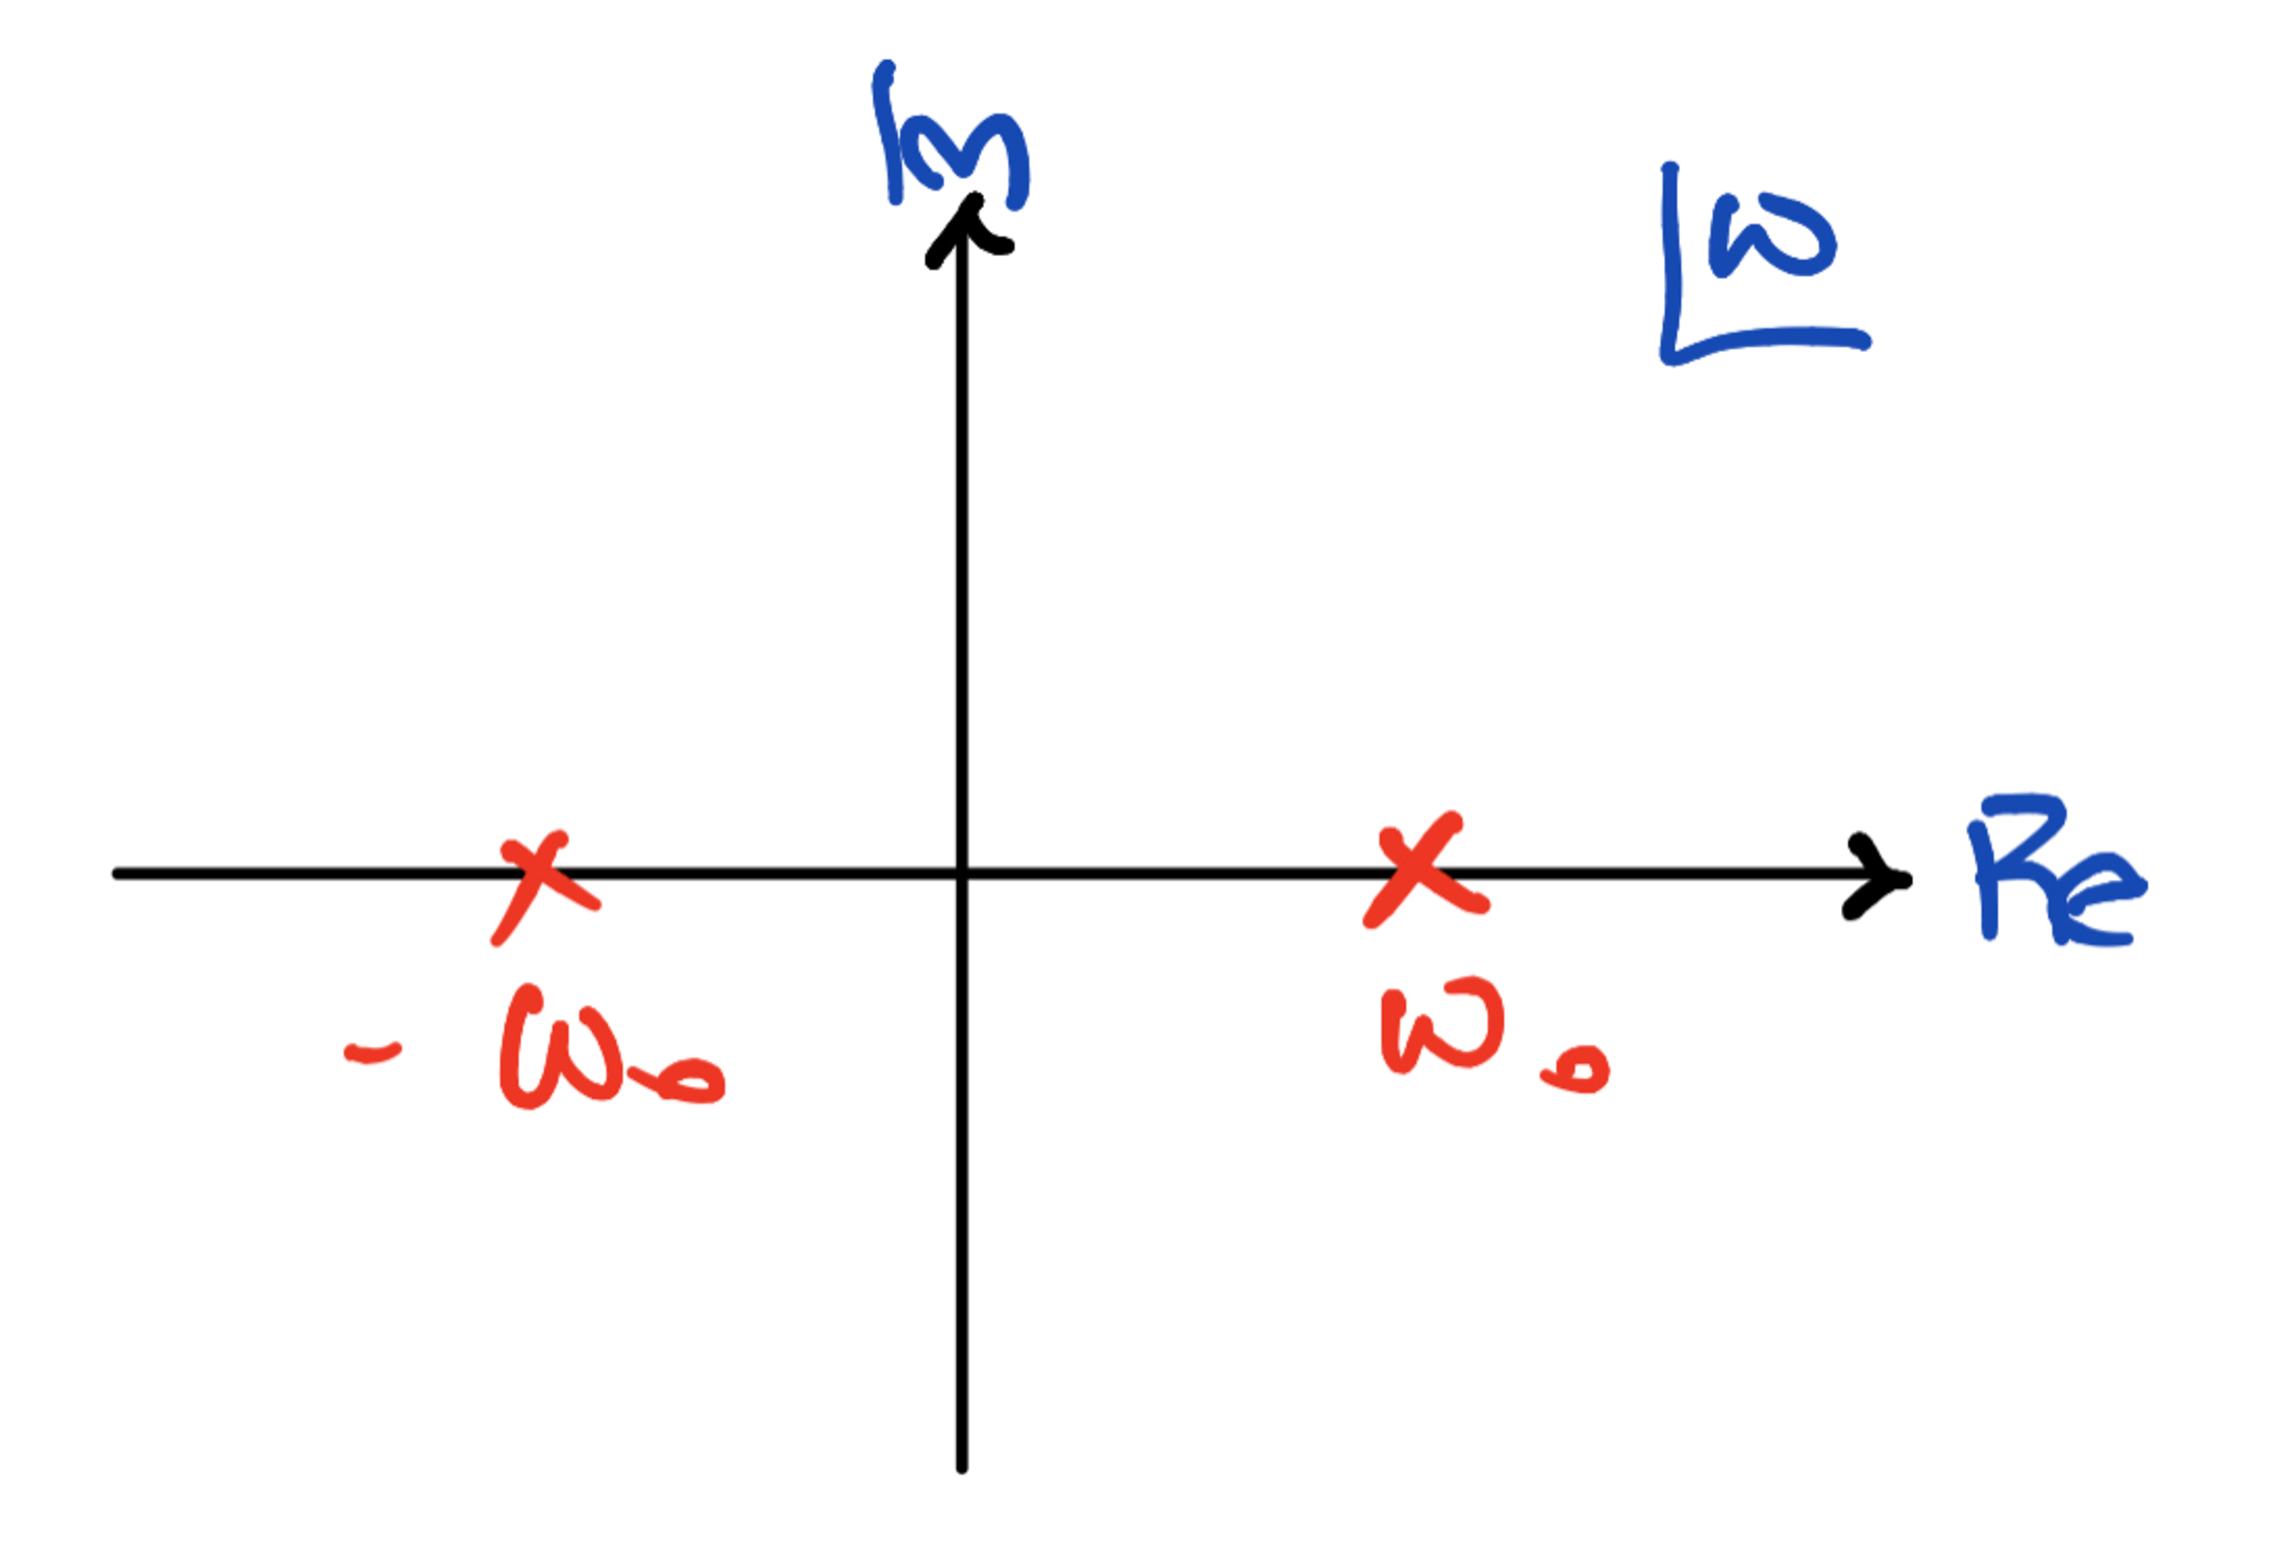
\includegraphics[width=.4\textwidth]{figures/Lec_2017_16_HO_Poles.pdf}
\end{center}
Please do take a brief moment to ponder at this existential crisis. This is an apparent failure of our theory---our calculation hits a pole, you get an infinity, and it's not clear what's going on. Rather than anguish, though, we should see if our theory is trying to tell us something. 

In order to figure out what's going on, let's do something wild. The poles on the real axis are in the way. Let's just move them out of the way by giving them small imaginary parts. Each pole can either be pushed above or below the real line:
\begin{center}
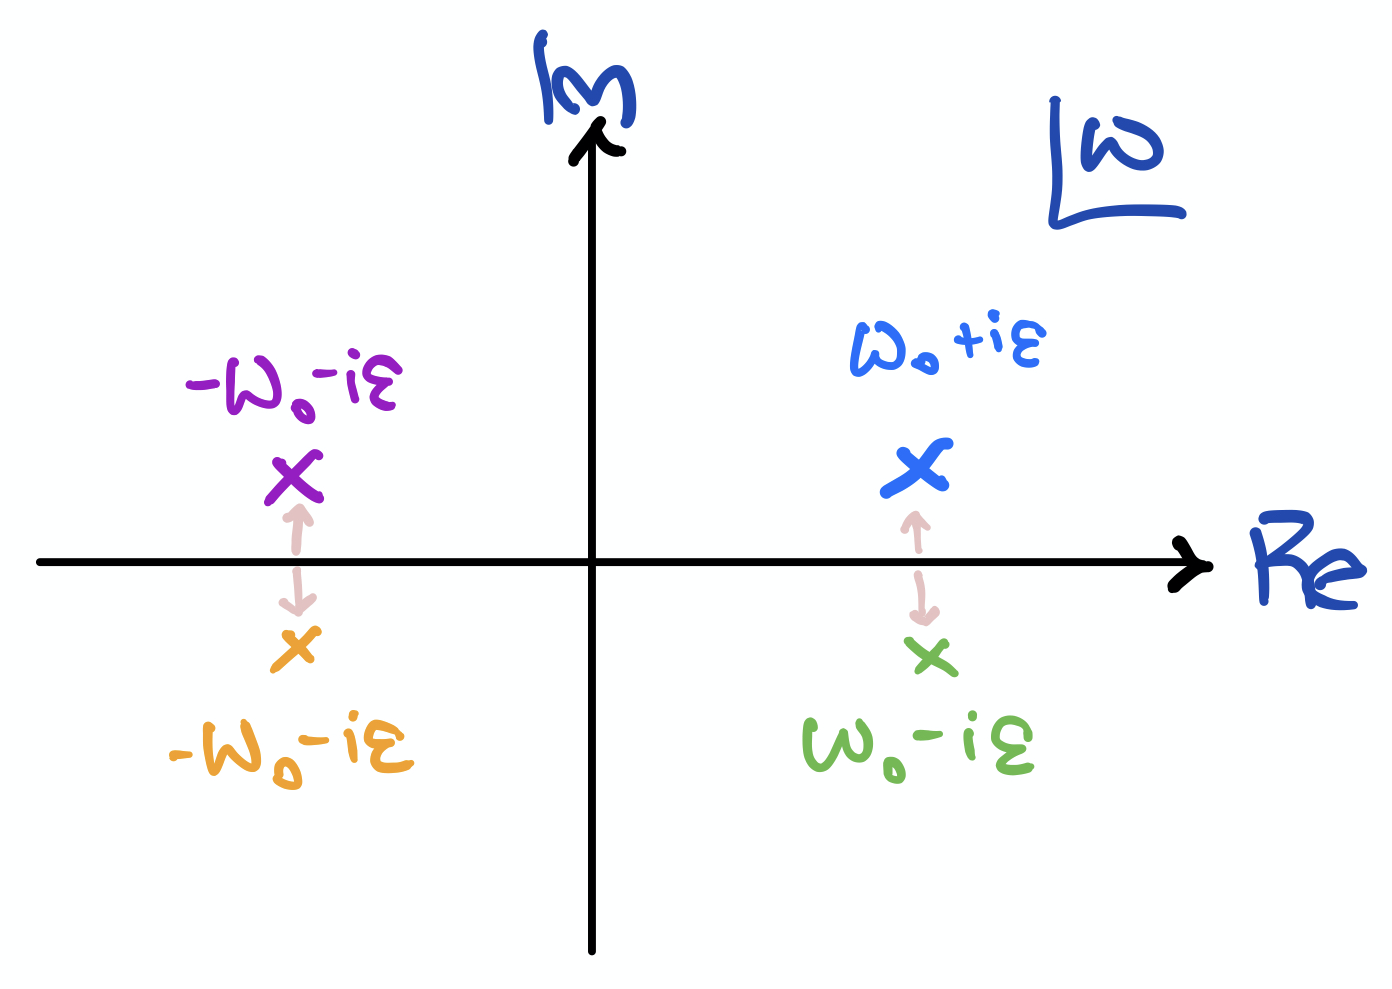
\includegraphics[width=.4\textwidth]{figures/Lec_2017_16_HO_PoleShift.png}
\end{center}
To be clear: are \emph{changing} the integral.\footnote{I have altered the poles. Pray that I do not alter them further.} We are exploring what happens when the expression \eqref{eq:G:HO:Fourier:Rep:t0:0} is changed, as if the poles were slightly complex the whole time. In other words, we are \emph{changing} the original differential operator, \eqref{eq:O:HO}. We're not yet motivating \emph{why} we want to do this; we'll justify it post-facto. For now, let's just be happy that our contours no longer bump into the poles. 

\section{Going under the poles?}
Let's try going under the poles, that is: let's push the poles into the upper half-plane with small imaginary parts:
\begin{center}
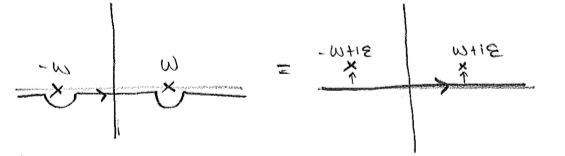
\includegraphics[width=.6\textwidth]{figures/Lec_2017_16_underpole.png}
\end{center}
This means that we have deformed the integrand \eqref{eq:HO:integrand:real:pole}:
\begin{align}
\frac{-e^{-i\omega t}}{(\omega - \omega_0)(\omega + \omega_0)}
&\to
\frac{-e^{-i\omega t}}{(\omega - \omega_0 - i\varepsilon)(\omega + \omega_0 - i\varepsilon)} \ .
\label{eq:HO:integrand:upper:poles}
\end{align}
To make it clear that we are treating $\omega$ as a complexified variable, let's write it as $z$:
\begin{align}
  \omega \to z \ .
 \end{align}
Now let's go through the exercise of performing the integral along the real line by using the residue theorem. To do this have to choose a contour that includes the real line. We have two options, $C_+$ and $\bar C_-$, where the bar reminds us of the orientation:
\begin{center}
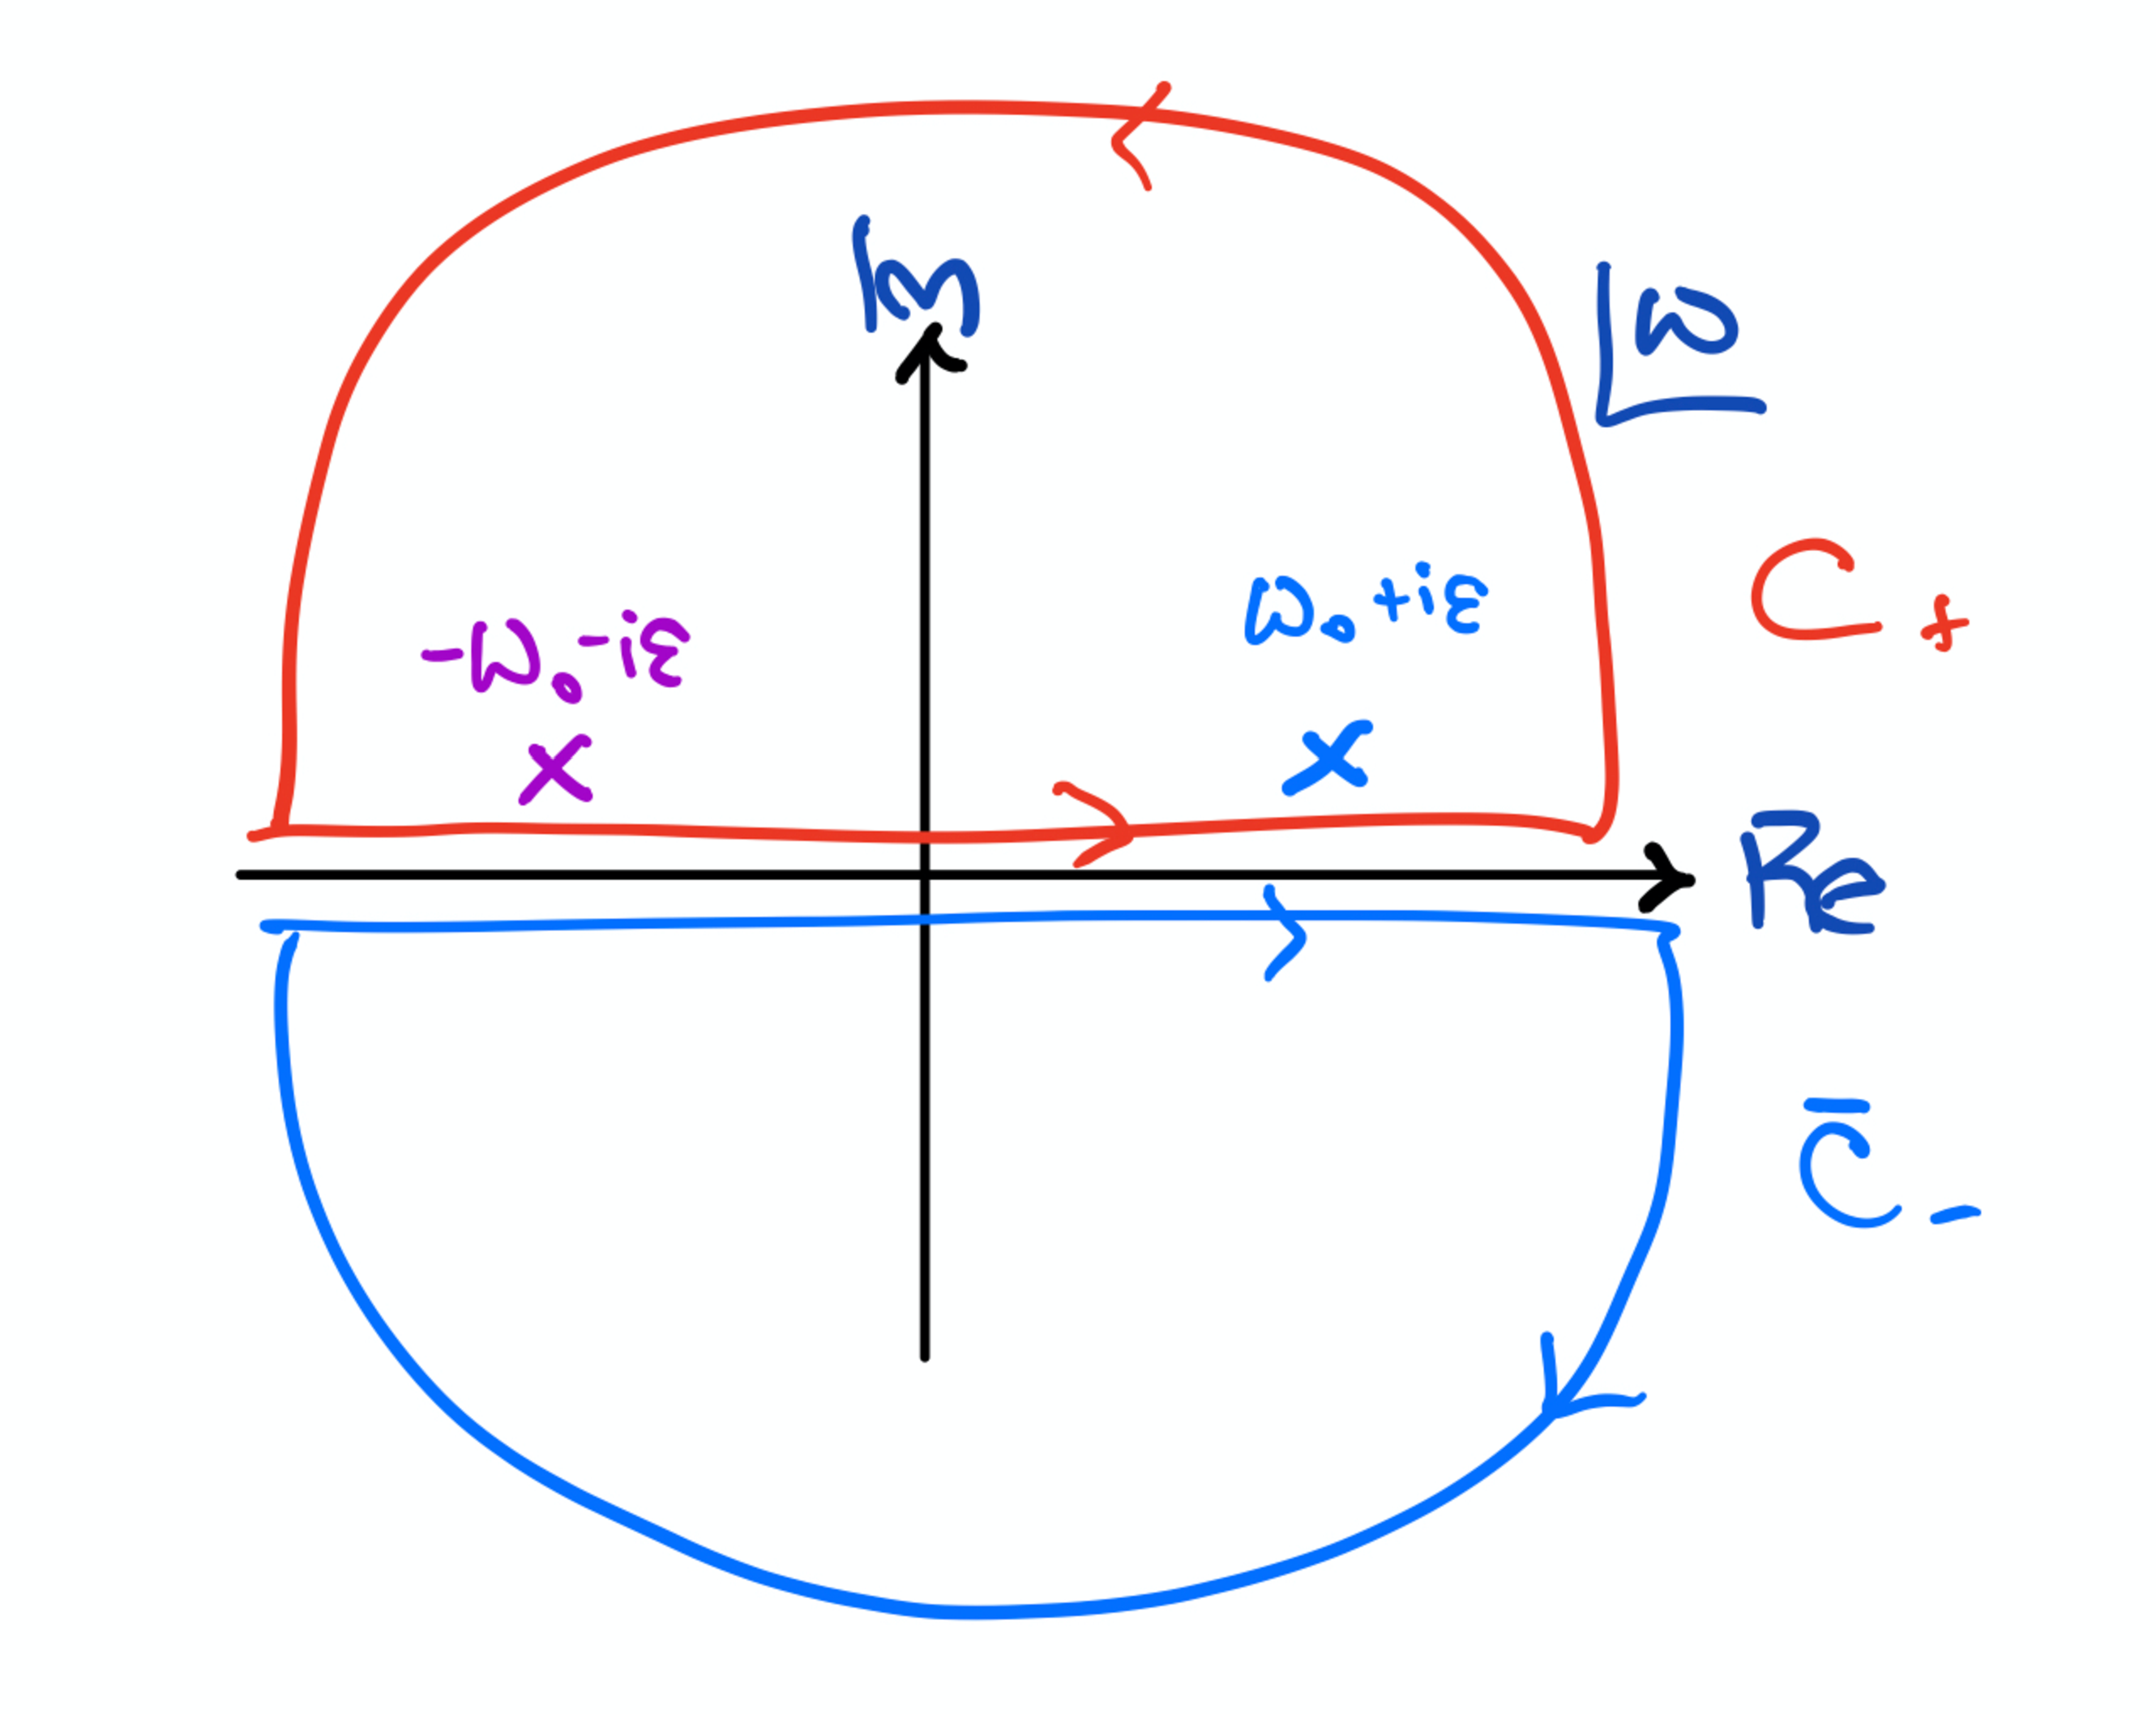
\includegraphics[width=.6\textwidth]{figures/Lec_2017_16_pokeup.pdf}
\end{center}
Which contour do we pick? Does it matter? (Yes!) The contours differ by whether the `large arc' has positive or negative real part. We can parameterize these arcs with respect to their real and imaginary parts:
\begin{align}
  z(\theta) &= R\cos\theta + i R\sin\theta \ ,
\end{align}
where for $C_+$ the arc is given by $\theta \in [0,\pi]$ while for $\bar C_-$ the arc is $\theta\in[0,-\pi]$. Note that the \emph{orientation} matters here---the $\bar C_-$ arc is moving in the clockwise direction.\footnote{Do people reading this even know why it is called `clockwise'? Analog clocks had mechanical arms that rotate.} The component in the imaginary axis is determined by $R\sin\theta$. Because $R$ is real and greater than zero, we have
\begin{align}
  \text{for $C_+$:}\, \sin\theta &> 0
  &
  \text{for $\bar C_-$:}\, \sin\theta &<0 \ .
  \label{eq:HO:which:contour}
\end{align}
%
How do we pick a contour? The criteria for completing the real line into a contour is that the integral along the contour vanishes, that way
\begin{align}
  \oint_C dz\, f(z) 
  = \int_{-\infty}^\infty dx\, f(x) + \lim_{R\to \infty} R \int_\text{arc} d\theta f(Re^{i\theta}) 
  = \int_{-\infty}^\infty dx\, f(x) \ .
\end{align}
And hence one can use the residue theorem to solve the contour integral on the left-hand side and relate it to the real integral on the right-hand side\footnote{I say `real integral' but of course the integrand \eqref{eq:HO:integrand:upper:poles} is now a complex quantity. The point is that we  only integrating along the real line.}. 
%
So which contour satisfies
\begin{align}
  \lim_{R\to \infty} R \int_\text{arc} d\theta 
  % f(Re^{i\theta})  
  \frac{-e^{-i(R\cos\theta + iR\sin\theta) t}}{(Re^{i\theta} - \omega_0 - i\varepsilon)(Re^{i\theta} + \omega_0 - i\varepsilon)}
  \to 0 \ ?
\end{align}
I was a little slick and chose to write $z = R\cos\theta + iR\sin\theta$ in the numerator while writing the more compact $z=Re^{i\theta}$ in the denominator. The convergence\footnote{I tend to say convergence, what I really mean is `vanishes as $R\to \infty$.'} of the integrand depends on the exponential factor in the numerator:
\begin{align}
  e^{-i(R\cos\theta + iR\sin\theta) t} = 
  e^{-iRt\cos\theta} e^{Rt\sin\theta} \ .
\end{align}
The first factor is purely oscillatory and is $\mathcal O(1)$ as $R\to\infty$. The second factor is either exponentially decaying or exponentially growing with large $R$. Convergence depends specifically on this second factor, $e^{-Rt\sin\theta}$. Since $R>0$, this depends on two things: the sign of $\sin\theta$ and the sign of $t$. The integral along the arc vanishes in the $R\to\infty$ limit when:
\begin{align}
  t > 0 \quad\text{and}\quad \sin\theta < 0 &
  &\text{or}&&
  t < 0 \quad\text{and}\quad \sin\theta > 0 \ .
  \label{eq:t:gtr:less:upper:poles}
\end{align}
Or in other words:
\begin{align}
  t>0 &\to \bar C_{-} 
  &
  t<0 &\to C_+ \ .
  \label{eq:t:sign:contour:HO}
\end{align}
% \begin{itemize}
%   \item $t>0$ and $\sin\theta > 0$ or
%   \item $t<0$ and $\sin\theta < 0$ \ .
% \end{itemize}
Recall that we have set $t_0 = 0$; if you did Exercise~\ref{eq:ex:Gtilde:with:t0:explicit}, you would know that restoring $t_0$ corresponds to $t\to t-t_0$ in the conditions above.

The Green's function equation \eqref{eq:Greens:func:as:inverse} is simply that $$\mathcal O_t G(t,t_0) = \delta(t-t_-)\ .$$ This tells us that the Green's function $G(t,t_0)$ is the \emph{response} measured at time $t$ to a $\delta$-function source at $t_0$. Thus the sign of $t-t_0$ corresponds to whether we are measuring the response \emph{before} or \emph{after} the cause. If you are like me, your eyes just lit up with joy. Something very exciting has happened: in this odd discussion about pushing around the poles of $\tilde G$, we have found that we were secretly talking about \emph{causality}.  

Before we progress, let's be clear: we expect that effects happen \emph{after} causes. This means that physical dynamics obey $t-t_0 >0$. A nice theory would tell us that you cannot have an effect before a cause. At the beginning of this course, we talked about locality as one of the motivating factors for why physical dynamics are described by differential operators. This was closely tied to the idea of causality, since non-local effects with spacelike separation can be non-causal in some reference frame. Perhaps amusingly---but beyond the scope of this course or my expertise---the notion of causality and locality in fundamental theories of nature continues to be a theme in cutting edge theoretical research. 

\paragraph{Causal propagation.}
For the specific case of $t>0$ (or $t-t_0>0$ if we restore $t_0$), we observe from \eqref{eq:t:gtr:less:upper:poles} that the integral \eqref{eq:HO:integrand:upper:poles} converges when $\sin\theta <0$. In other words, for times \emph{after} the initial cause at $t_0=0$, the appropriate contour is $\bar C_-$. 
\begin{exercise}
What is the value of the contour integral 
\begin{align}
  \oint_{\bar{C}_-} dz\, \frac{-e^{-i z t}}{(z - \omega_0 - i\varepsilon)(z + \omega_0 - i\varepsilon)} \ ?
\end{align}
Hint: you shouldn't have to do any work.
\end{exercise}
% The contour integral above vanishes along the arc when $t>0$, so it is the correct contour when doing the Fourier transform to get $G(t)$ from $\tilde G(\omega)$. However, 
This contour encloses no poles. No poles means no residues. This means that the contour integral vanishes and the Fourier transform vanishes. In other words, 
\begin{align}
  G(t>0) &= 0 \ .
  \label{eq:HO:G:t:gtr:0:zero}
\end{align}

\begin{example}
The statement that $G(t>0)=0$ should make you sad and possibly upset. This means that there is \emph{no} effect that happens after some cause at $t_0=0$.
\end{example}

\paragraph{Acausal propagation.} By now you see the writing on the wall. Something perverse has happened: after a $\delta$-function disturbance, information is not traveling forward in time because $G(t)=0$ for $t>0$. This, in turn, was self-evident in because for $t>0$, we were required to take the $\bar C_-$ contour in order that the contribution of the arc vanishes. At this point, you must feel the dread of what's coming next. If we take the $t<0$ case in \eqref{eq:t:gtr:less:upper:poles}, we are forced to take the $C_+$ contour. This contour indeed picks up poles and so we expect it to be non-zero. Thus we find that $G(t<0) \neq 0$, which is awful because this $t<0$ corresponds to an \emph{effect that happens before the cause}. 

\begin{exercise}
Taking $t_0=0$ for simplicity, show that the exact result for the acausal Green's function is
\begin{align}
  G(t<0) &= \frac{-1}{\omega_0}\sin\omega_0t \ .
  \label{eq:HO:G:t:less:0:nonzero}
\end{align}
Hint: the relevant residues are $\pm e^{\pm i\omega_0t}/2\omega_0$ \ .
\end{exercise}
You should \emph{do} the above exercise as practice for the main contour integral of this entire course. If you are stuck, you can keep reading these notes.\footnote{By now you should know that learning physics requires \emph{doing} physics. Reading/watching someone else do physics is one of the least efficient ways of improving yourself.} 

To help you along, let me even set up the integral for you. We start with $G(t)$ in \eqref{eq:HO:integrand:real:pole}, where we rewrote the integrand in \eqref{eq:G:HO:Fourier:Rep:t0:0} to make the pole structure clear. We then said that we wanted to push the poles off the real line. This \emph{changes} the physical problem, but we'll worry about what that means later. In this case, we move the poles into the upper half-plane so that each pole has a small imaginary part. The poles are then located at $\pm \omega_0 + i \varepsilon$. The resulting integral is:
\begin{align}
  G(t) &= 
  \int_{-\infty}^\infty \frac{d\omega}{2\pi} 
  \frac{-e^{-i\omega t}}{(\omega - \omega_0-i\varepsilon)(\omega + \omega_0-i\varepsilon)} 
  \ .
\end{align}
Complete the real integral into a contour integral; we'll re-label our variables to remind us that we're in the complex plane, $\omega\to z$. The contour that we select, $C_+$, came from the $e^{-i\omega t}$ factor. The result is:
\begin{align}
  \oint_{C_+}
  \frac{dz}{2\pi} 
  \frac{-e^{-iz t}}{(z - \omega_0-i\varepsilon)(z + \omega_0-i\varepsilon)}
  =&\phantom{+} 
  \int_{-\infty}^\infty \frac{d\omega}{2\pi} 
  \frac{-e^{-i\omega t}}{(\omega - \omega_0-i\varepsilon)(\omega + \omega_0-i\varepsilon)} 
  \nonumber
  \\
  &
  + 
  \cancel{
  \lim_{R\to\infty} \int_{0}^\pi \frac{Rd\theta}{2\pi} 
  \frac{-e^{-i(R\cos\theta + i R\sin\theta)t}}{(Re^{i\theta} - \omega_0-i\varepsilon)(Re^{i\theta} + \omega_0-i\varepsilon)} 
  }
  \label{eq:HO:G:integral:adv:1}
  \\
  &=
  2\pi i \sum_{z_\pm=\pm\omega_0+i\varepsilon} \text{Res}_f(z) \ ,
  \label{eq:HO:G:integral:adv:2}
\end{align}
where $f$ is understood to be the integrand. 
%
From here you should be able to read off the result. Confirm that we can take the $\varepsilon\to 0$ limit; this tiny shift was only there to tell us that the poles live in the upper half-plane.

\paragraph{Advanced propagator.}
The causal ($t>0$) and acausal ($t<0$) cases in \eqref{eq:HO:G:t:less:0:nonzero} and \eqref{eq:HO:G:t:gtr:0:zero} respectively may be combined into a single expression:
\begin{align}
  G_\text{adv}(t) &= \frac{-1}{\omega_0}\sin(\omega_0t) \Theta(-t) \ ,
  \label{eq:HO:G:adv:theta}
\end{align}
where we use the Heaviside step function
\begin{align}
  \Theta(x) = 
  \begin{cases}
  1 & \text{if}\; x>0\\
  0 & \text{if}\; x<0 \ .
  \end{cases}
  \label{eq:Heaviside:Theta}
\end{align}
\begin{exercise}
Check the overall sign. I keep screwing this up. You are henceforth responsible for the overall sign and I absolve myself of any mistakes due to this sign.
\end{exercise}
This is the \textbf{advanced} propagator. Even though `advanced' is often a positive adjective when applied to your progress\footnote{I once read a story about a particle physicist who started a conversation with a stranger on the plane. The stranger explains, ``My son is really quite brilliant. He's studying physics at an Ivy league university.'' The physicist says, ``Oh, how nice. You know, I'm a physicist.''  The stranger then asks what kind of physics, to which the physicist says ``I study elementary particles.'' The stranger responds with, ``Ah yes. Well, my son studies advanced particles.'' I no longer remember where I read this story, but I can attest to meeting people like this.} In this context, however, `advanced' is a \emph{bad} word. It means \emph{acausal}: the cause comes \emph{after} the effect. This does not make any sense, and we reject this as non-sense. 

After an appropriate amount of indignant disdain, we can reflect on how the heck we got here\footnote{If your response is \emph{Christmas! Christmas eve last year}, then I applaud your taste in musical theater.}. We make two observations:
\begin{enumerate}
\item After checking all of our work, the main conclusion from this non-sense result is that our approach of pushing the poles \emph{up} into the upper half-plane must have been wrong. We see that the position of the poles tells us about the causality of the system. By pushing the poles off the real axis, we have imposed a sense of causality in time. We should see what happens when we push the poles \emph{down} into the lower half-plane. 

\item Even though the \emph{physics} of advanced propagator is utter rubbish because it breaks causality, we also appreciate that it is a perfectly reasonable \emph{mathematical} solution. The harmonic oscillator dynamics encoded in our differential operator $\mathcal O_t$ is symmetric with respect to time-reversal symmetry\footnote{The behavior of our models under $t\to -t$ is a powerful diagnostic for understanding our physical theories. One of my friends was in a pub the night before lecture and some of the pub regulars, who knew he was a physicists, asked him what he was lecturing on the next day. He said he was going to talk about reversing the direction of time, to which they cautiously responded: `\emph{... we can do that??}'}. The `physical' interpretation is analogous to seeing a bunch of ripples starting at the edges of a pond that move inward until they reach a singularity ($\delta$-function!?) at which point the pond spits out a small pebble. 
\end{enumerate}


\begin{exercise}
At this point, you should be able to solve the case of the causal Green's function without any additional guidance. In fact, without doing any work, you should see that by pushing the poles down into the lower half plane, the propagator will be causal. With a little bit of thought, you may be able to write the analog of \eqref{eq:HO:G:adv:theta}, the retarded Green's function,
%\footnote{In the same way that `advanced' means something different colloquially versus for physics, we use this word very carefully. One of my friends in graduate school was an international student who liked to make physics puns. At some point she playfully admonished late arriving undergraduates for being `retarded,' which required quite a bit of care to clarify the situation to everyone involved.}, 
without doing any work. You should still proceed to calculate $G_\text{ret}(t)$ the `honest way.' We walk  through it together in the next subsection. 
\label{ex:retarded:G:HO}
\end{exercise}

\section{Going over the poles}

Assuming that you have completed Exercise~\ref{ex:retarded:G:HO}, you have figured out the main result of this course\footnote{Do the exercises. I've come to appreciate how annoying it is to come up with meaningful exercises, rather than rote calculations. At some point there's a phase transition in education where exercises are no longer just `practice' but are pedagogical tools to make sure your brain knows how to \emph{think} physics rather than just \emph{read} physics. To say it differently, as my undergraduate advisor once told me: you should do every single exercise problem you can. If you're short on time, just focus on the ones that you cannot do.}. However, because this example is so important, let's go ahead and walk through it together. We push the poles down into the lower half-plane by giving them a small imaginary part, $-i\varepsilon$.

\begin{center}
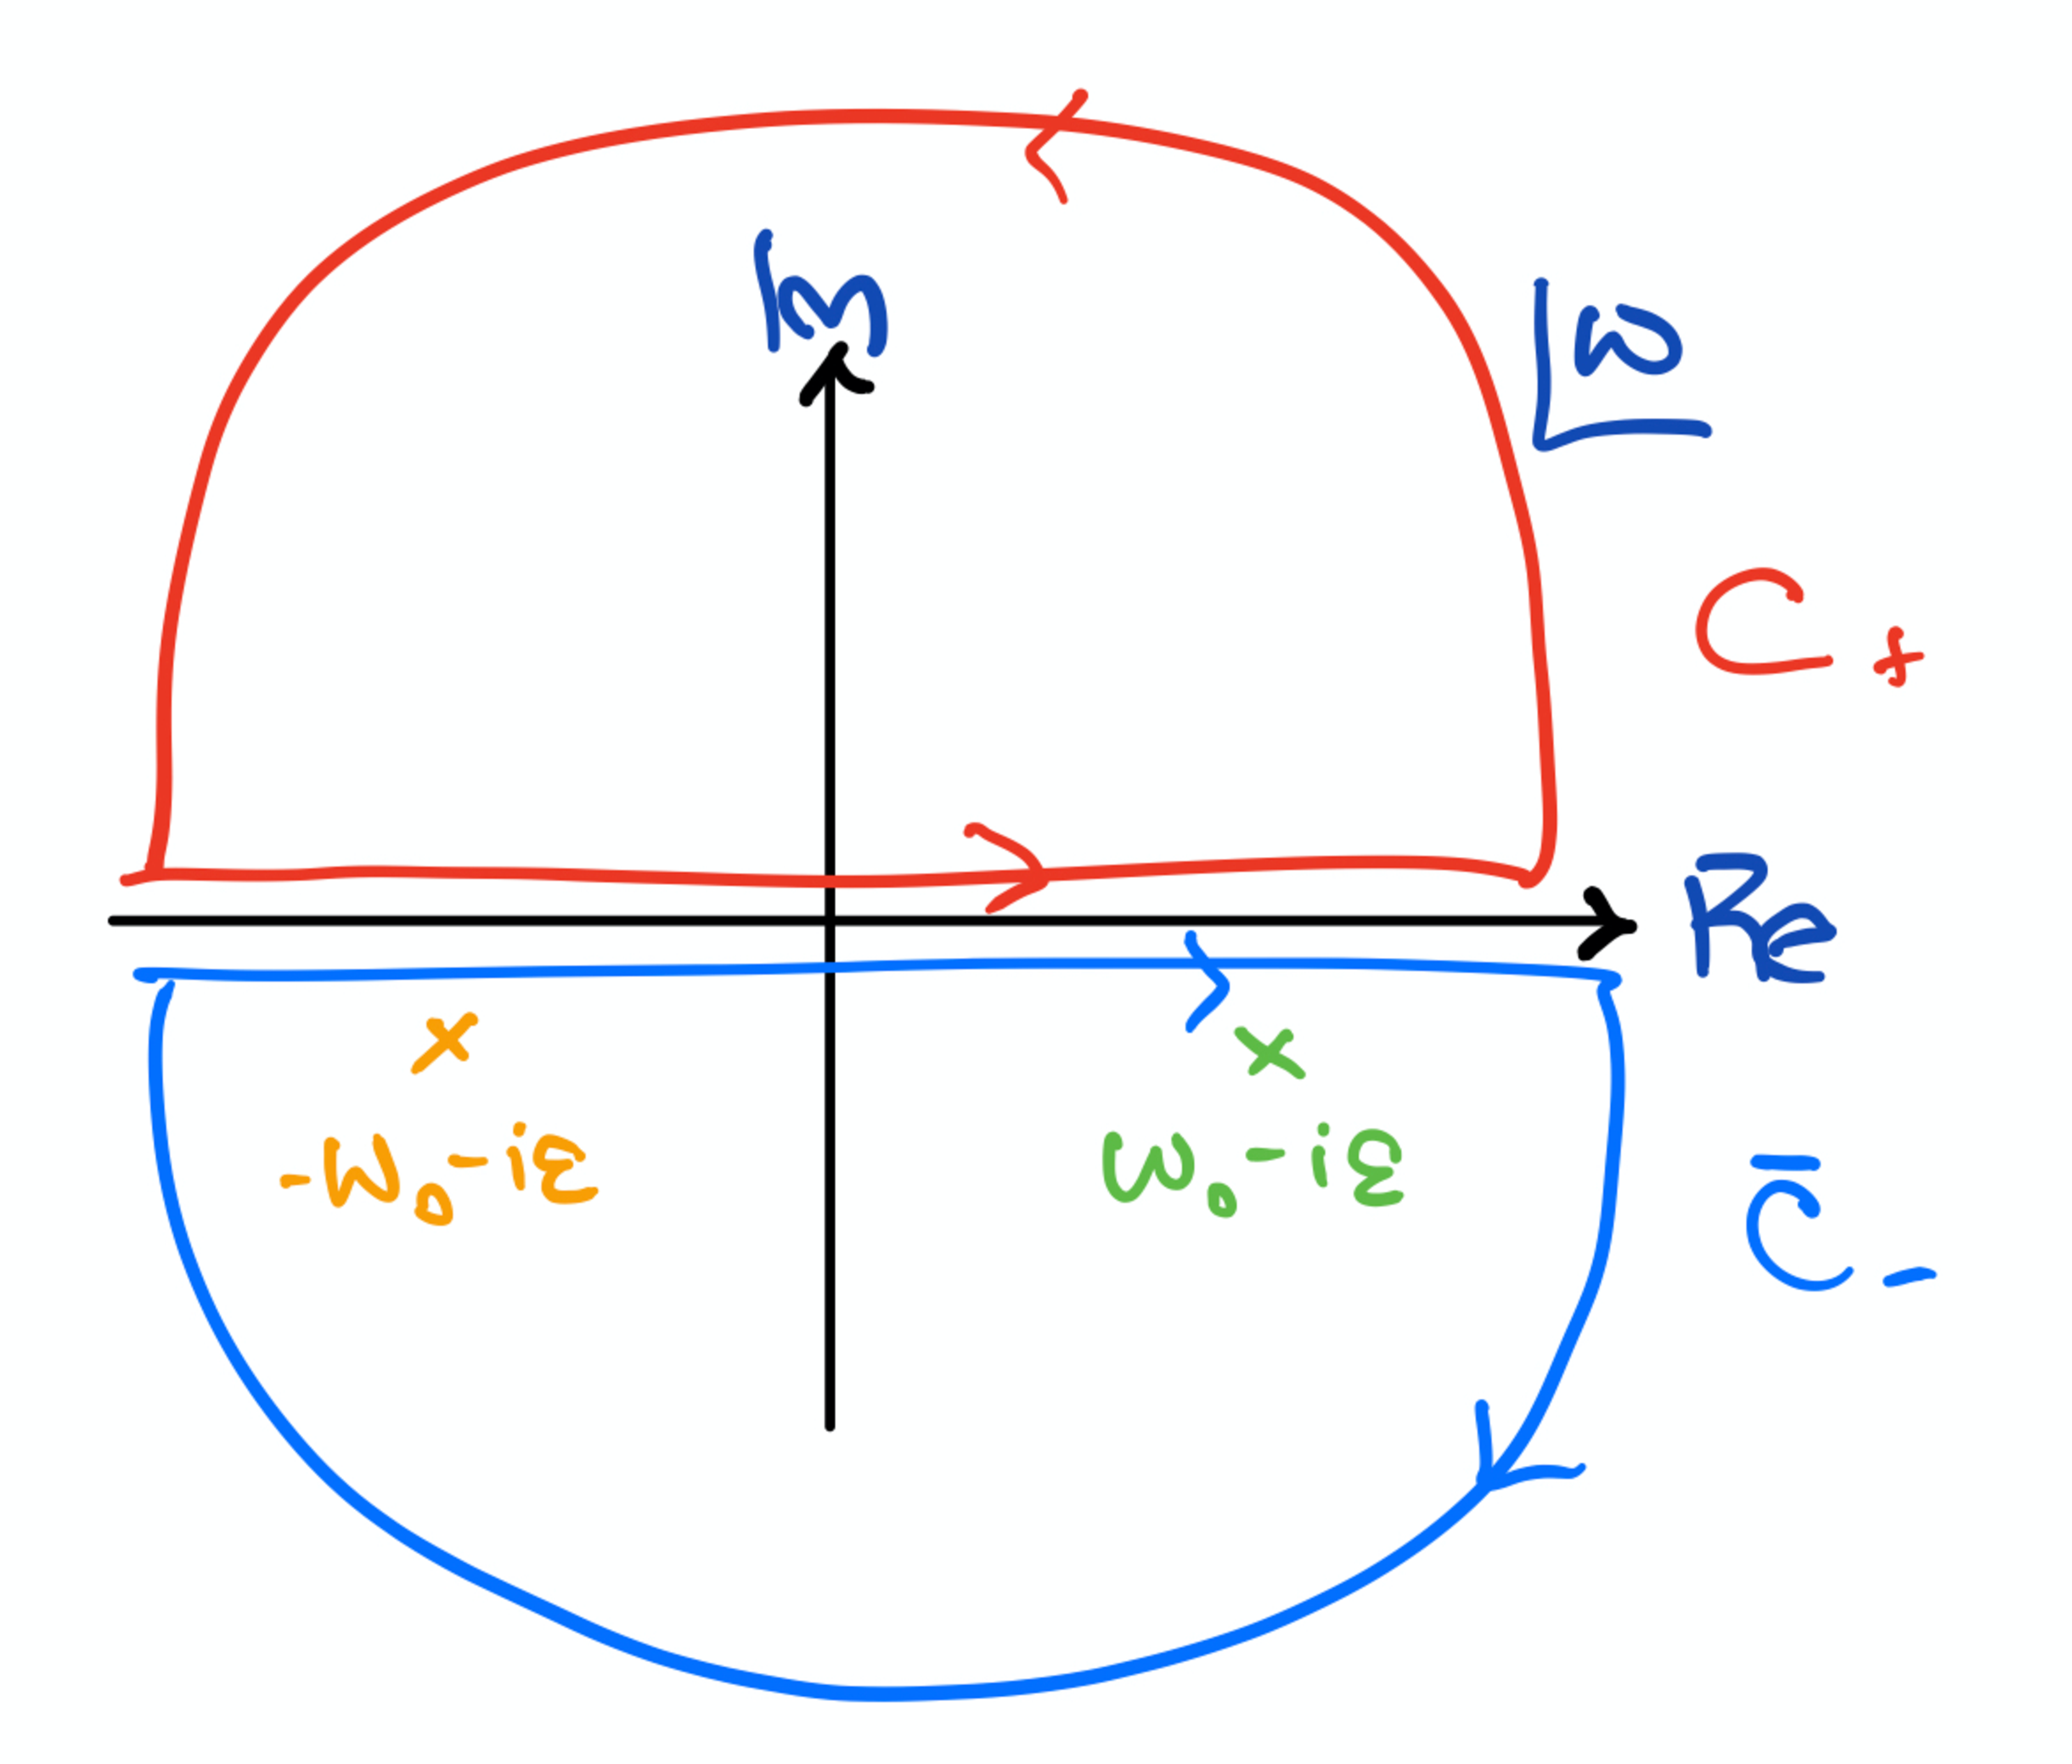
\includegraphics[width=.4\textwidth]{figures/Lec_2017_16_pokedown.pdf}
\end{center}

The integral is exactly the same, except the sign of $\varepsilon$ has changed. 
\begin{exercise}
Pop quiz! Unlike the advanced Green's function where we gave the poles a small positive imaginary part, we have now given the poles a small \textbf{negative} imaginary part. How do we assign the contours $C_+$ and $\bar C_-$ to the cases $t>0$ and $t<0$?
\end{exercise}
Did I fool you? The poles may have moved, but the way that we pick contours does not change! The appropriate contour is an unambiguous choice determined by the $e^{-i\omega t}$ factor in the integrand. Thus we \emph{still} have the \emph{same}contour choices in \eqref{eq:t:sign:contour:HO}:
\begin{align}
  t>0 &\to \bar C_{-} 
  &
  t<0 &\to C_+ \ .
\end{align}
What has changed is that now the $\bar C_{-}$ contour encloses poles, whereas the $C_+$ contour encloses no poles. This clearly tells us that the integral over $\omega$ (or its complexificaion $z$) is zero for $t<0$, which means we do not have acausal propagation: 
\begin{align}
  G(t<0) &= 0 \ .
  \label{eq:HO:G:ret:acausal}
\end{align}
Hooray! Signals do not arrive before they are sent.

What about the causal propagation? Remember that $\bar C_{-}$ has a negative orientation. To keep our signs clear, let's write the integral as negative a contour $C_-$  which has the positive orientation: 
\begin{align}
  \oint_{\bar C_-} = -\oint_{C_-} \ .
\end{align}
We can go ahead and do the integral over $C_-$ using the residue theorem. We're simply re-doing \eqref{eq:HO:G:integral:adv:1} and \eqref{eq:HO:G:integral:adv:2} with $\varepsilon\to -\varepsilon$. Writing $f(z)$ to be the integrand, we have:
\begin{align}
  G(t>0) =& 
  -\frac{1}{2\pi} \oint_{C_-}dz\, f(z)
  \\
  =&
  2\pi i \times -\frac{1}{2\pi} 
  \left(\text{Res}_f(\omega_0) + \text{Res}_f(-\omega_0)\right)
  \\
  =& \frac{1}{\omega_0}\sin(\omega_0 t) \ .
\end{align}
Combining this with \eqref{eq:HO:G:ret:acausal} using the Heaviside $\Theta$-function \eqref{eq:Heaviside:Theta} gives the \textbf{retarded Green's function}:
\begin{align}
  G_\text{ret}(t) &= 
  \frac{1}{\omega_0}
  \sin(\omega_0 t)
  \Theta(t) \ .
  \label{eq:HO:Gret:sin:theta}
\end{align}
\begin{exercise}
Restore $t_0\neq 0$ in the above equation for the retarded Green's function.
\end{exercise}
By the way, we will often use the word \textbf{propagator} in place of Green's function. This is because the Green's function propagates information from the source to the observation point\footnote{This is especially clear when solving linear differential equations for which the Green's function represents an exact solution. For non-linear problems, one typically resorts to a perturbation expansion of linear propagators with order-by-order corrections in non-linearity. %This is what Feynman diagrams are: lines represent propagators, which are Green's functions for the linear part of the dynamical equation. The vertices represent non-linearities which must be treated as a Taylor series about a partition function.
}. 

\begin{exercise}
Check the overall sign of the retarded Green's function.  Confirm that the nonzero part of the retarded Green's function ($t>0$) has the opposite sign as the nonzero part of the advanced Green's function ($t<0$). Confirm that this sign difference is due to the orientation of the contour $C_+$ versus $\bar{C}_-$.
\end{exercise}

\section{Other choices? The Feynman Propagator}

We introduced the advanced $G_\text{adv}$ and retarded $G_\text{ret}$ Green's functions. These are both Green's functions for the harmonic oscillator, but for technically different versions of the harmonic oscillator where the differential operator $\mathcal O_t$ has been tweaked to make it slightly complex. We always take the complex part to zero at the end, but we have nudged the poles of the Fourier integrand over a bit and discovered that these have implications on the causality of the Green's function. Clearly the Green's function that we want for most classical applications is the retarded Green's function; this one reflects an effect that happens after the cause.

However, we may as well also explore alternative pole-pushing options. Consider the following mixed prescription:
\begin{center}
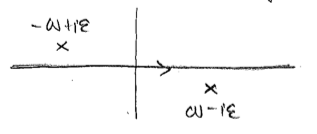
\includegraphics[width=.6\textwidth]{figures/Lec_2017_16_Feynman.png}
\end{center}
Here one pole is pushed up and the other is pushed down. We'll only focus on the case of $+\omega_0$ being pushed into the lower half-plane and $-\omega_0$ being pushed into the upper half-plane. I'll leave it to you to figure out the implications of the converse choice.
\begin{example}
Even before we do any of the work, you should identify why this is strange. The exponential factor of the Fourier integrand determines which contour we select. This, in turn, is based on the sign of $t$ and connects to our notion of causality. By splitting the poles like this, we see that there is a non-zero contribution to \emph{both} causal and acausal propagation. What's even more curious, we no longer get the combination of two complex exponentials that gives a (real) sine. Thus the Green's function is manifestly complex. Curious!
\end{example}
We call this the Feynman propagator, $G_F$, which should make you suspect that this choice is not just some mathematical curiosity but actually has physical significance. The result is:
\begin{align}
  G_F(t>0) &= \frac{i}{2\omega_0} e^{-i\omega_0 t}
  &
  G_F(t<0) &= \frac{-i}{2\omega_0} e^{i\omega_0 t} \ .
  \label{eq:HO:G:Feynman}
\end{align}
\begin{exercise}
Prove \eqref{eq:HO:G:Feynman} using the techniques demonstrated in this section.
\end{exercise}
This Green's function turns out to be the correct choice in quantum field theory. Even if you don't know what quantum field theory is, you can guess from the name that this makes sense:
\begin{enumerate}
\item The `quantum' implies that maybe complex numbers aren't so odd. In fact, the $e^{\pm i\omega_0 t}$ looks a lot like $e^{i\hat H t}$, the time-evolution operator. Indeed, frequencies and energies have the same dimension once you throw in the appropriate factors of $\hbar = 1$.
\item The word `field' implies something like a continuum. Continua are represented by a bunch of nearest-neighbor connected springs---in other words, they are naturally represented as coupled harmonic oscillators\footnote{This fact should be better presented in the standard undergraduate curriculum. I recommend Howard Georgi's lectures on waves.}.
\end{enumerate}
What the Feynman propagator/Green's function represents two things, depending on the sign of $t$:
\begin{enumerate}
\item $t>0$: a plane wave moving forward in time with positive energy, $G_F \sim e^{-i\omega t}$. This seems totally fine. The fact that $G_F$ is imaginary is not a big deal, since it now represents something like a wavefunction in quantum mechanics. 
\item $t<0$: a plane wave moving \emph{backward in time} with  with \emph{negative energy}, $G_F \sim e^{-i(-\omega) t}$. This is the suspicious case: note the `double negative' of moving backward in time and having negative energy.
\end{enumerate}
You may know the resolution of the $t<0$ solution since it's a popular story in physics. Dirac found that the solution to the dynamical equation for relativistic electrons contained negative energy electrons moving backward in time. These corresponded to currents of negative charge moving backward in time, which you can hand-wave into understanding as a \emph{positive} charge moving \emph{forward} in time. In other words, rather than describing negative energy electrons moving backward in time, these states correspond to positive-energy positrons moving forward in time. Thus we have a theoretical invitation to the existence of anti-particles.

\begin{flipcomment}
For those interested in particle or nuclear physics, you may also want to notice that the particle and the anti-particle propagators differ by complex conjugation. This is related to the idea that charges reflect some complex nature of the particles. The geometric description of electrodynamics is a $U(1)$ fibration of spacetime. What this means is that every field is allowed to have a complex phase: the $U(1)$ refers to rephasing symmetry, $z\to e^{i\phi} z$. The other familiar forces of fundamental physics are described by the generalization to what is called $SU(N)$ where an $N$-vector of particles $\Psi^i$ transforms under the $N\times N$ special unitary matrix $U^i_{\phantom i j}=\exp(i\phi^a T^a)^i_{\phantom i j}$ so that $\Psi^i \to U^i_{\phantom i j} \Psi^j$. The matrices $T^a$ are called the `generators' of these $N$-dimensional rephasings. For the case $SU(2)$, the $T^a$ are simply the three Pauli matrices, $\sigma^a$ and the $N$-vectors are essentially two-component spinors. The anti-particles are Hermitian conjugates of the particles $\Psi$.
%\label{footnote:U1:SUN}. 
\end{flipcomment}

\section{Feynman Green's Function and the Convergence of the Path Integral}

This section is purely `for culture'. We present a qualitative discussion of how one could have anticipated the Feynman propagator from the perspective of the path integral formulation of quantum mechanics. While path integrals are outside the scope of our course, the overall story here is helpful to see how a theory predicts an equation of motion. The Fourier components of the Feynman Green's function are:
\begin{align}
  \tilde G(k) &=
  \frac{-1}{
  \left[k-(\omega_0 -i\varepsilon)\right]
  \left[k-(-\omega_0 + i\varepsilon)\right]
  }
  =
  \frac{-1}{
  k^2 - \omega_0^2 + 2i\varepsilon \omega_0
  }
  \ .
  \label{eq:Feynman:G:tilde}
\end{align}
Define the small imaginary part to be $2i\epsilon \omega_0 \equiv 2i\delta$. This is just a small, dimensionful quantity.\footnote{A `small dimensionful quantity' implicitly makes reference to another dimensionful quantity against which `smallness' is measured. In this case, it is the resonant frequency $\omega$. Ultimately, the `small' thing is the dimensionless $\varepsilon$.}  This is what we would expect from a Lagrangian:
\begin{align}
  L = \frac{1}{2}\dot q^2 - \frac{1}{2}\left(\omega_0^2 - 2i \delta\right)q^2 \ .
\end{align}
Note: this replacement should be `obvious': we just take $\omega_0^2 \to \omega_0^2 - 2i\delta$.
\begin{exercise}
Check that the equation of motion from this Lagrangian indeed gives a differential operator whose Green's function has Fourier components \eqref{eq:Feynman:G:tilde}.
\end{exercise}
Since the the Lagrangian is related to the action, $S$, by $S=\int dt\, \mathcal L$, one can integrate the $\dot x^2$ term by parts to write:
\begin{align}
  S = -\int dt \, \frac{1}{2}
  q 
  \left[\left(\frac{d}{dt}\right)^2 + \omega_0^2 - 2i\delta \right]
  q 
  =
  -\int dt \, \frac{1}{2}
  q 
  \left[\mathcal O_\text{HO} - 2i\delta \right]
  q  \ ,
  \label{eq:HO:S:Feynman:quad}
\end{align}
where $\mathcal O_\text{HO}$ is the original harmonic oscillator differential operator that we started with in \eqref{eq:O:HO}. This shows us that the Feynman prescription for pushing poles around corresponds to adding a small imaginary part to the harmonic oscillator Lagrangian. This is a little weird since the resulting operator is clearly not Hermitian.

If you're familiar with statistical mechanics or quantum field theory, you may know that the fundamental object is neither the Lagrangian nor the action\footnote{... and is definitely not the Hamiltonian; sorry condensed matter folks and Lin-Manuel Miranda fans.}, but actually the path integral, $Z$ which is defined as an integral over all possible functions $x(t)$:
\begin{align}
  Z &= 
  \int \mathcal Dq(t) \, e^{iS[q]}
  = 
  \int \mathcal Dq(t) \, e^{iS_\text{HO}[q] - \delta q^2} \ .
\end{align}
Here $\mathcal Dx$ is just the measure of the path integral. For discretized space, it corresponds to $\mathcal Dx\sim dq(t_0)\,dq(t_1)\, dq(t_2)\cdots$. The harmonic oscillator action $S_\text{HO}$ is real and thus $e^{iS_\text{HO}}$ oscillates and the path integral doesn't converge. By adding the $- \frac{\delta}{2} q^2$ term to the action we are imposing a small perturbation that forces the integrand to converge for very large values of $x(t)$. With this factor the path integral is well defined. If we approached the harmonic oscillator assuming that path integral is sufficiently convergent\footnote{Physically this is saying that these extreme path configurations should not contribute since the path that minimizes the action should be far away from these cases; so we're just helping the theory focus on the part of the path integral that matters.} and plugging in some factor to force this convergence, then we can run this argument backward and `deduce' the Feynman prescription for the Green's function.

If everything in this subsection is a bit boring, then here's what you should know. This discussion gives us a hint of where all of our physical differential equations come from. The equations of motion that define a theory come from a variational principle with respect to some action. 
\begin{exercise}
[optional] What is the action (Lagrangian, Hamiltonian, whatever...) that yields Maxwell's equations? Note that curiously, you only get half of Maxwell's equations from an action principle. The other half comes from ideas in Section~\ref{sec:stokes:theorem:aside}. For a discussion by a well-known \acro{UCR} mathematical physicist, see \emph{Gauge Fields, Knots And Gravity} by Prof.~John Baez.
\end{exercise}
We then recall that our actions (Lagrangians, Hamiltonians, ...) tend to be \emph{local} function(al)s, so it makes sense that they can be written as a derivative expansion. The actions depend on particles/fields, say\footnote{I'm deliberately changing notation from $x(t)\to q(t)$. This is important because we will eventually want to treat $x$ and $t$ as spacetime coordinates rather than $x(t)$ as `the position of \emph{the} particle at time $t$.' This unfortunately notational confusion tends to be one of the conceptual hurdles in field theory.} $q(t)$. If we write out the leading terms of the action with respect to $q(t)$ you get something like
\begin{align}
  S[q] &= \int dt \, (\text{const.}) + \mathcal O_1 q(t) + \mathcal O_2 q^2(t) + \mathcal O_3 q^2(t) + \cdots
\end{align}
where the $\mathcal O_i$ are differential operators. We can ignore the constant. Usually the $\mathcal O_1$ term doesn't show up, so let's ignore that too; you can remove it by redefining the particle\footnote{The linear term tells you that you're probably not defining the `zero' of your field sensibly. Amusingly, this is closely related to the Higgs phenomenon that gives known fundamental particles most of their mass.}. The $\mathcal O_2 q^2$ term can be integrated by parts. The details of the integration by parts depend on the details of the derivatives in $\mathcal O_2$, but one can write typically write this term as
\begin{align}
  \mathcal O_2 q^2(t) &\equiv - q(t) \mathcal O_\text{quad} q(t) \ ,
\end{align}
which is in the form that we used in \eqref{eq:HO:S:Feynman:quad}. When we derive the equation of motion by varying the action, we end up with
\begin{align}
  -\mathcal O_\text{quad} q(t) = 0 \ ,
\end{align}
where I am probably assuming that $\mathcal O_\text{quad}$ is Hermitian if we want to be technical. The main observation here is that this is a \emph{linear} differential equation. Linear differential equations in physics come from the quadratic pieces of actions. Since we argued that the linear piece is usually not there and we know that the constant piece corresponds to a shift in the vacuum energy (that's \emph{usually} not physical\footnote{Damn you, dark energy.}), then this quadratic piece of the action is the \emph{lowest order} contribution to the action in an expansion of the particle $q(t)$ with respect to the vacuum ($q(t)=0$). The higher-order terms correspond to differential equations that are \emph{not} linear since the variation of that term contains $q^2(t)$. So yes, even though the mathematical structures here are a bit more fancy, let us state out loud that all of our main differential equations in physics basically boil down to taking the leading term in a Taylor expansion. Typical for physicists, eh?

\section{Example: The Damped Harmonic Oscillator}
 
 At this point we are happy that the physical solution to the classical harmonic oscillator is the retarded Green's function, $G_\text{ret}(t)$. There is an unphysical solution, the advanced Green's function, $G_\text{adv}(t)$ that reflects a mathematical symmetry of the theory (time-reversal invariance) but is otherwise not of physical interest. Finally, there is a solution that makes sense for quantum physics, the Feynman Green's function, $G_\text{F}(t)$, which is complex but reflects the existence of anti-particles. Each of the above cases came from \emph{almost} the same harmonic oscillator differential operator, $\mathcal O$, except the operators were slightly deformed so that its poles were off of the real line in the complex momentum plane. We took the limit where this deformation goes to zero, but not until after we've exploited those deformations to do the Fourier integral using the residue theorem. We came to appreciate that the infinitesimal nudge in the imaginary direction was telling us something about the causality of the harmonic oscillator.

 We can understand the nature of this imaginary push by looking at the \emph{damped harmonic oscillator}. The dynamical equation for the damped harmonic oscillator is
 \begin{align}
  \mathcal O_\text{DHO} x(t) = \ddot{x}(t) + 2\gamma\dot x(t) + \omega_0^2 x(t) = F(t) \ ,
 \end{align}
 where $\gamma$ is the \textbf{damping coefficient} and $F(t)$ is a driving force.
 \begin{exercise}
 What are the dimensions of the damping coefficient, $\gamma$?
 \end{exercise}
 
 \paragraph{Back of the envelope version.}
 Before doing anything quantitative, we can guess the behavior. A non-zero $\gamma$ suppresses the response $x(t)$ to the source $F(t)$. Unlike an idealized instrument, a guitar string has non-zero damping and the vibrations get smaller the longer you wait after plucking it. If we imagine a plane wave\footnote{I keep calling $e^{-i\omega t}$ a plane wave because I'm thinking of the generalization to spacetime. For now there are no transverse directions, so of course $e^{-i\omega t}$ is really just a wave.} $x(t)\sim e^{-i\omega t}$ and ask what this wave looks like far away from the source, $F(t)\to 0$, then the differential equation reads:
 \begin{align}
  -\left(\omega^2 +2i\gamma \omega - \omega_0^2\right)e^{-i\omega t} &= 0 \ .
 \end{align}
 The solution for the plane wave's frequency $\omega$ is
 \begin{align}
  \omega = \omega_R - i\gamma \ , \label{eq:DHO:back:envelope:poles}
 \end{align}
 where for $\gamma^2 \ll \omega_0^2$, $\omega_R \approx \omega_0$ is the frequency.  Plugging $\omega$ back into our plane wave gives
 \begin{align}
  x(t) = e^{-i\omega_R t}e^{-\gamma t} \ .
 \end{align}
 The first factor is the usual plane wave. We recognize the $\exp(-\gamma t)$ as an exponential suppression that causes the plane wave to get rapidly smaller for times larger than $1/\gamma$. There are a few lessons:
 \begin{enumerate}
 \item In \eqref{eq:DHO:back:envelope:poles} we have implicitly but decisively bought into the idea of a complex frequency. The interpretation of this complex frequency is that the real part is the usual oscillation and the imaginary part corresponds to damping.

 \item The solution \eqref{eq:DHO:back:envelope:poles} corresponds to finding the poles of the Fourier integrand; recall, for example, \eqref{eq:G:HO:Fourier:equation:integrals}. So damping has something to do with the imaginary part of the poles in the complex plane.

 \item Because the position of the pole in the imaginary direction is related to the \emph{causality} of the theory, we have now connected `damping' to causality in a round-about way.

 \item When we derived the retarded Green's function $G_\text{ret}(t)$ that describes the classical, ideal harmonic oscillator, we took $i\varepsilon\to 0$. For the damped harmonic oscillator the corresponding value is $i\gamma$, which we keep finite\footnote{Here's a funny bit of linguistics in our discipline. Any physical quantity is naturally not-infinite, so it seems silly when physicists make a point to call something `finite.' You would think that this is in contrast to that quantity being infinite. In fact, when physicists say \emph{finite} what they really mean is \emph{not zero}, which is quite different from `not infinite.'}\footnote{Actually, there's a second aside I'd like to make in the footnotes. Jim Holt has an excellent essay, ``The Dangerous Idea of the Infinitesimal'' about how mathematicians struggled with the idea of infinitesimal quantities. The essay is reproduced in his volume \emph{When Einstein Walked with G\"odel}.}; it has some physical significance after all.

 \item The exponential notation for the Fourier transform made all of this very easy: we just let $\omega$ be complex in $e^{-i\omega t}$ and we are able to capture the physics of oscillations and damping. If we had used trigonometric functions then we'd have a bunch of $\sinh$ or $\cosh$ floating around and the convergence would not be so clear.
 \end{enumerate}
 
 \paragraph{More carefully.} Let's go through the steps to derive the Green's function for the damped harmonic oscillator properly. The Green's function equation is
 \begin{align}
  \left[
  \left(\frac{d}{dt}\right)^2
  + 2\gamma \frac{d}{dt}
  + \omega_0^2
  \right]
  G(t)
  &=
  \delta(t) \ ,
 \end{align}
 where we've again set $t_0 = 0$. It is easy at this stage to restore\footnote{There is a theorem that $G(t,t')$ only depends on $|t-t'|$ under reasonable assumptions. You should be able to argue this on physical grounds.} $t_0$ by taking $t\to (t-t_0)$. Plugging in the Fourier representations for the $t$-dependence,
 \begin{align}
  G(t) &= \int \dbar \omega \, e^{-i\omega t}\tilde G(\omega)
  &
  \delta(t) &= \int \dbar \omega e^{-i\omega t} \ ,
 \end{align}
 then gives:
 \begin{align}
  \tilde G(\omega) &=
  \frac{-1}{\omega^2+2i\gamma\omega -\omega_0^2} \ .
 \end{align}
 The poles occur at 
 \begin{align}
  \omega_\pm &= \frac{-2i\gamma \pm \sqrt{-4\gamma + 4\omega_{0^2}}}{2}
  = \pm \sqrt{\omega_0^2 - \gamma^2} - i \gamma \equiv \pm \omega_R - i\gamma\ .
  \label{eq:DHO:poles}
 \end{align}
 \begin{example}
 The poles in \eqref{eq:DHO:poles} have a real part as long as $\omega_0^2 > \gamma^2$. What does it mean when $\omega_0^2 < \gamma^2$? This is the observation that the damping is stronger than the characteristic oscillation frequency, $\omega_0$. Thus the system is properly describe by an exponentially suppression because it never has a chance to oscillate.\footnote{This is one of the magical things about $B$ mesons. $B$ mesons are really nice systems whose characteristic oscillation frequency (between $B$ and anti-$B$ mesons) and characteristic decay width are roughly of the same order of magnitude. When we produce $B$ mesons at, say, the LHCb experiment, we get to observe the decays (imaginary part) of these mesons after $\sim 1$ oscillation which gives a powerful tool for studying matter--anti-matter asymmetry.\label{footnote:B:meson}}
 \end{example}
 Assuming $\omega_0^2 > \gamma^2$, then we may identify $\omega_R = +\sqrt{\omega_0^2 - \gamma^2}$ and the poles may be written as $\pm \omega_R - i\gamma$. This looks a \emph{just} like the pole prescription for the retarded Green's function of the ideal harmonic oscillator with $\omega_0\to \omega_R$ and $i\varepsilon\to i\gamma$. In fact, we can just follow all of the same steps that we did for the retarded Green's function:
 \begin{enumerate}
 \item The poles are in the lower half-plane of $\omega$. This means that the propagator is automatically causal (it's the retarded, not the advanced Green's function).
 \item The exponential factor $e^{-i\omega t}$ in the Fourier integral determines the convergence of the integrand and hence how we complete the contour. For $t>0$ we close the contour on the lower half-plane and pick up these poles in the residue theorem. For $t<0$ we close the contour on the upper half-plane; since there are no poles here, the Fourier integral vanishes.
 \item We end up with our own version of \eqref{eq:HO:Gret:sin:theta} with $\omega_0\to\omega_R$ except we need to account for the finite $\gamma$. 
 \end{enumerate}
 The only substantial difference between the damped harmonic oscillator and the ordinary harmonic oscillator is that $\omega_\pm$ contains a non-negligible imaginary part. The contour integral takes the form:
 \begin{align}
  \oint_C dz \,
  \frac{-e^{-izt}}{
  \left(z-\omega_+\right)
  \left(z-\omega_-\right)
  }
  =&
  \phantom+ 
  2\pi i\left(\text{Res}_f\omega_+ + \text{Res}_f\omega_-\right)
  \\
  =&
  -2\pi i\left[
  \frac{e^{i\omega_+t}}{\omega_+-\omega_-}
  +
  \frac{e^{i\omega_-t}}{\omega_--\omega_+}
  \right]
  \\
  =&
  -2\pi i
  \frac{e^{i\omega_+t} - e^{i\omega_-t}}{\omega_+-\omega_-}
  \\
  =&
  -2\pi i \frac{e^{-i\gamma t}}{2\omega_R}
  \left(e^{i\omega_Rt} - e^{-i\omega_Rt}\right)
  \\
  =&
  \pi \frac{e^{-i\gamma t}}{2\omega_R}
  \sin(\omega t)
   \ .
 \end{align}
 Plugging this into the full solution---which involves keeping track of which contour integral is non-zero and where the factors of $2\pi$ belong---we find:
 \begin{align}
  G(t) = \frac{e^{-\gamma t}}{\sqrt{\omega_0-\gamma^2}} \sin\left(\sqrt{\omega_0^2-\gamma^2} t\right) \Theta(t) \ .
  \label{eq:DHO:G:sin:theta}
 \end{align} 
 \begin{exercise}
Compare and contrast \eqref{eq:DHO:G:sin:theta} to \eqref{eq:HO:Gret:sin:theta}. Why is the general form the same? How do you explain the differences? What is the behavior for $\omega \gg \gamma$, $\omega \ll \gamma$? What does it look like if you restored $t_0$?
 \end{exercise}
 The key observation that we have from this discussion is that the choice of pushing the poles into the lower half plane---which we found was critical for a causal Green's function---is actually physically motivated. Any \emph{physical} oscillating system actually has some small amount of friction (or the appropriate generalization) that causes it to not only oscillate, but also decay. 
 \begin{exercise}
 In quantum mechanics the time evolution operator is $e^{i\hat H t}$. Maybe there's a minus sign in there, I don't remember and I don't really care. It is important that this operator is unitary, or else probabilities are not preserved in time. However, there are plenty of physical systems (say, the $B$ meson in footnote~\ref{footnote:B:meson}) that \emph{are} described my non-Hermitian Hamiltonians, i.e.~non-unitary time evolution operators. Reason tells us that the form of the time-evolution operator should be $e^{i\hat H t}e^{-\gamma t}$, since probabilities less than one make more sense than probabilities bigger than one. What is the physical interpretation of this non-unitary time evolution? Hint: this has to do with the notion that our theory (our Hamiltonian) models something in nature, but it not model \emph{all} of the relevant pieces nature for a given problem.
 \end{exercise}
 At this point in my note I have the following written:
 \begin{quote}
 \emph{I took 5 weeks of physics 231 and all I have is this one stupid Green's function.}
 \end{quote}
 
 
 
\chapter{The Harmonic Oscillator in More Dimensions}



In most graduate courses, we examine simple examples where we can focus on understanding the physics. We then leave it to you to generalize to the horrible real-world scenarios that you will encounter in your other graduate courses and research. There is one generalization that we should take time to do properly together: the shift from one dimension to multiple dimensions. This is the shift from working with functions of time to functions \emph{spacetime}. Equivalently, the harmonic oscillator converts into a wave.
%
Keep in mind that we are not doing any special relativity, even though borrow notation from special relativity\footnote{There was once a professor teaching electrodynamics who used notation informed by relativity. Some of the condensed matter students complained the class is about electricity and magnetism, not relativity. The professor replied: just where do you think magnetism comes from?}. 




\section{The `harmonic oscillator' in spacetime}
The second derivative in higher-dimensional Euclidean space is the Laplacian, $\nabla^2= \partial_x^2 + \partial_y^2 +\cdots$. But when you combine space and time (Minkowski space), there's the famous relative minus sign\footnote{At this level the minus sign is a convenient convention, but we know that the second derivative should really be relativistically invariant: $\partial^2 = \partial_\mu \partial^\mu$.}:
\begin{align}
  \frac{d^2}{dt^2}
  \to 
  \frac{1}{c^2}
  \frac{\partial}{\partial t}^2
  -
  \frac{\partial^2}
  {\partial \vec x^2} \ ,
\end{align}
where $\partial/\partial\vec x = \nabla$ is the gradient. The overall sign is a convention. Against all of my hard-developed instincts for natural units, I have replaced the explicit value of $c$ so that the operator makes sense dimensionally: each term has powers of inverse length squared. In what follows I am likely to make mistakes with the factors of $c$.\footnote{As my adviser used to say: ``If you think there may be a sign error or a factor of two error, then your homework is to fix those errors.'' In this case, if you think there's a missing factor of $c=1$, I am not even sure if I would even acknowledge that it is actually an error.} 

In (1+1)-dimensional of spacetime\footnote{The (1+1) notation means one dimension of space, one dimension of time.} the second derivative is $\partial^2 = c^{-2} \partial_t^2 - \partial_x^2$. That looks familiar, doesn't it? The minus sign tells us that if we move forward in time a little bit, but `look backward' in space, then the function does not change. The description of the state at time $t-\delta t$ and position $x-\delta x$, subject to $\delta x = c\delta t$, is the same as the state at time $t$ and position $x$. 
%
This means that the information was propagated \emph{forward} in space as time also moves forward. This is exactly what we expect from a wave. We recall that the solution to second derivative differential equations are usually trigonometric functions or their exponential counterparts. We further recall that `plane waves' are described with the same funny minus sign:
\begin{align}
  f(t) \sim \sin (\omega t - kx) \ .
  \label{eq:plane:wave}
\end{align}
From this you can read off that the plane wave velocity is $\omega/k$. Of course, you already knew that from dimensional analysis. 

\begin{exercise}
This is a great place to reflect on phase versus group velocity. I should probably write such a discussion into a future version of this notes. \flip{To do.} In the meanwhile, one of my favorite puzzles is the following (perhaps apocryphal) story.\footnote{I think I first heard this story from Tony Zee's lectures at the African School for Theoretical Physics in 2004. He posed this as an \emph{obvious} problem in dimensional analysis. I do not think I properly appreciated the `obvious' aspect until about 15 years later while preparing this course. It was not---and still is not---obvious to me at all.} During the second world war, an admiral wanted to be able to use reconnaissance photographs of ships to determine their velocities. The admiral knew that given data about the ships' positions and velocities, one could extrapolate where those ships are going and when they will arrive. Because ships leave a wake behind them, the admiral figured that a clever physicist should be able to determine a ship's velocity based on the angle of the wake behind the boat.

In deep water, this is called a Kelvin wake. You also see this when watching ducks on the river.\footnote{Not everyone has a chance to watch battleships from a spy plane, but it turns out plenty of universities are situated near rivers where generations of the mathematically inclined could reflect on physical phenomena. One could just sit by the water and think. I suspect this is the reason why Cambridge has such a historically strong fluid dynamics department. Anyway, I used to watch the ducks swimming in the stream near my old Ph.D institution. There were also geese around. I would not watch the geese. I suspect they also leave a Kelvin wake, but what I know with certainty is that geese leave behind gigantic goose shits that make it unpleasant to sit by the water.} The key `aha' moment for understanding the Kelvin wake is that the relevant model is one where the key restoring force comes from gravity---these wakes are formed by \emph{gravity} waves. Do not confuse this with \emph{gravitational waves}, which are quite different. By neglecting surface tension, we find that the phase velocity is $\sqrt{g/k}$, where $k$ is the wave number ($e^{ikx}$). The group velocity (that carries energy) is $d\omega/dk$, where $\omega=\sqrt{gk}$ is the angular frequency. Thus the group velocity is half the phase velocity. 

Using a geometric argument, show that the angle of the Kelvin wake is $\sin^{-1}(1/3)$. The book by Stone \& Goldbart has a nice discussion.\footnote{See also \url{www.itp.uni-hannover.de/fileadmin/itp/emeritus/zawischa/static_html/KWake.html}} Even before jumping into the construction, you should wonder where the ratio 1:3 shows up in the problem. 
\end{exercise}
% A good exercise: phase and group velocity; see appell or cahill


\section{Green's functions for multidimensional spaces}
Our `harmonic oscillator' equation becomes:
\begin{align}
  \left[\frac{1}{c^2}
      \frac{\partial}{\partial t}^2
      -
      \frac{\partial^2}
      {\partial x^2}
      -
      \frac{\partial^2}
      {\partial y^2}
      -
      \frac{\partial^2}
      {\partial z^2}
    \right]
    \varphi(\vec{x},t) = \rho(\vec{x},t) \ .
    \label{eq:phi:wave:eq}
\end{align}
Huh, that looks familiar, doesn't it? We've chosen variables so that this looks just like the wave equation for the scalar potential $\varphi$ subject to a charged source $\rho$ in electrodynamics! In fact, you know how this works. There are three more equations that correspond to the vector potential:
\begin{align}
  \left[\frac{1}{c^2}
      \frac{\partial}{\partial t}^2
      -
      \frac{\partial^2}
      {\partial x^2}
      -
      \frac{\partial^2}
      {\partial y^2}
      -
      \frac{\partial^2}
      {\partial z^2}
    \right]
    \vec A(\vec{x},t) = \vec j(\vec{x},t) \ .
    \label{eq:A:wave:eq}
\end{align}
Now let's go through a series of questions about \eqref{eq:phi:wave:eq} and \eqref{eq:A:wave:eq} to make sure we're on the same page. 
\begin{enumerate}
\item \textbf{Are these differential equations still linear?} Yes. Remember what it means to be linear! $\mathcal O(f+g) = \mathcal Of +\mathcal Og$, for example.
\item \textbf{Are we worried that there are multiple arguments?} Not really. The functions now depend on $t$ and $\vec{x}=(x,y,z)$. You went from an infinite dimensional `vector space' to a still-infinite dimensional vector space\footnote{You can pontificate about whether this infinity is `bigger.' It doesn't really make a difference.}. You can also mumble reassuring words to yourself, perhaps recalling how in prior encounters with the wave equation you've perhaps separated your functions into single-argument factors, $\Psi(t,x) = T(t)X(x)$, or something like that.
\item \textbf{How many equations are there?} There are \emph{four}\footnote{Obligatory TNG reference: \url{https://www.youtube.com/watch?v=wjKQQpPVifY}} equations. There is an equation for $\phi$ and one equation for each component of $\vec A$. In fact, we typically bundle this all up into a four-vector $A_\mu=(\varphi, \vec A)$.\footnote{For now this is just a bundling, so you may argue that it's not obviously a \emph{vector}. The fact that $\varphi$ and $\vec{A}$ transform into each other upon performing a boost is something we learn from physical observations. Alternatively, the identity of $A_\mu$ as a vector (technically, a one-form) is imposed by the mathematical structure---but that mathematical structure was adopted after the empirical progress in the 1800s.}
\item \textbf{How many differential operators are there?} Just one. There is only \emph{one} differential operator, $\partial^2$. It acts on different components of $A_\mu$, but it's the same wave operator acting on each component. 
\item \textbf{... so how many equations are there, really?} All four equations are essentially the same equation with different state functions and different sources. So it's really just one class of differential equation.
\end{enumerate}
Okay, here's the really important one. I'm going to put it in a box to make sure you pay really close attention. Please answer the following question before reading on:
\begin{flipcomment}
\centering
How many Green's functions are there?
\end{flipcomment}
Do we need a Green's function for each component of $A_\mu$? Do we need a Green's function for each dependent variable, $x^\mu = (ct,x,y,z)$? \emph{No}! There is only \emph{one} differential equation, and thus there is only \emph{one} Green's function. 

Let's see how this works. Suppose you have a differential equation in multiple variables,
\begin{align}
  \mathcal O_{\vec{x}} f(\vec{x}) = s(\vec{x}) \ .
\end{align}
Let's say that $\vec{x}=(x_1, \cdots, x_N)$, so that we're working in $N$-dimensional space. Suppose you are given the Green's function $G(\vec{x},\vec{x}')$ for $\mathcal O_{\vec{x}}$. This means that $G$ satisfies the Green's function equation
\begin{align}
  \mathcal O_{\vec{x}} G(\vec{x},\vec{x}') = \delta^{(N)}(\vec{x}-\vec{x}') \ ,
\end{align}
where the $N$-dimensional $\delta$-function is simply the product of one-dimensional $\delta$-functions in the expected way:
\begin{align}
  \delta^{(N)}(\vec{x}-\vec{x}') 
  &=
  \delta(x_1-x_1')\delta(x_2-x_2')\cdots\delta(x_N-x_N') \ .
\end{align}
The solution to the above differential equation is
\begin{align}
  f(\vec{x}) &= \int d^N\vec{x}'\,  G(\vec{x},\vec{x}') s(\vec{x}') \ ,
\end{align}
which you can check by acting on both sides with $\mathcal O_{\vec{x}}$.




\section{Relativistic Notation}

Let's borrow some four-vector notation from special relativity. Nothing that we're doing is based on special relativity, but the fact that it pops out for free is telling. Our indices $\mu$ run over four values which we take to be $\mu = 0,1,2,3$ corresponding to timelike (0) and spacelike (1,2,3) directions. Some objects are naturally defined with an upper index, like $x^\mu = (ct,x,y,z)$. You can lower these indices using the metric, $\eta_{\mu\nu}=\text{diag}(1,-1,-1,-1)$. This means that for some vector $v^\mu$,
\begin{align}
  v^2 \equiv v^\mu v_\mu 
  = c^2(v^0)^2 - (v^1)^2 - (v^2)^2 - (v^3)^2 \ .
 \end{align}
 More importantly, this means that the four-vector of partial derivatives, which is naturally a lower-index object, squares to:
 \begin{align}
   \partial^2\equiv
  \partial_\mu \partial^\mu 
  &= 
  \frac{1}{c^2}
      \frac{\partial}{\partial t}^2
      -
      \frac{\partial^2}
      {\partial x^2}
      -
      \frac{\partial^2}
      {\partial y^2}
      -
      \frac{\partial^2}
      {\partial z^2} \ .
 \end{align}
The placement of the $c^2$ factors should be clear from dimensional analysis. We see that indeed the wave operator is the natural generalization of the harmonic oscillator in spacetime. We won't actually be raising and lowering indices, but we want to be clear that there's a natural `dot product' that includes the relative minus sign between spatial and temporal components.

The states and sources in our system are the (four-)vector potential $A_\mu$ and the current $j_\mu$: 
\begin{align}
  A_\mu &= (\varphi, \vec{A})
  &
  j_\mu &= (\rho, \vec{j}) \ .
\end{align}
The four equations for the vector potential are
\begin{align}
  \partial^2 A_\mu = j_\mu \ .
\end{align}
That's one equation for each value of $\mu$, but each equation has the \emph{same} differential operator $\partial^2$. Our task is to find the Green's function for this operator in spacetime. The Green's function equation is
\begin{align}
  \partial^2 G(x,x') &= \delta^{(4)}(x-x') \ ,
  \label{eq:wave:eq:Greens:eq}
\end{align}
where we write $x$ and $x'$ to mean \emph{four}-vectors with \emph{components} $x^\mu$ and $(x')^\mu$. Given a current $j_\mu(x)$, the vector potential is the solution to the wave equation which integrates over all of the current (source) positions:
\begin{align}
  A_\mu(x) &= \int d^4x' \, G(x,x') j_\mu(x) \ .
\end{align}
Observe that $G$ has two arguments, $x$ and $x'$, but no indices. The two arguments correspond to the observation point $x$ and the source point $x'$. The integral over $d^4x'$ means we're accounting for sources from all positions and all times\footnote{This should remind you of starlight that is emitted a long time ago ($t'$) in a galaxy far, far away ($\vec{x}'$ that we we observe today $(t,x)$.}. We have not specified our choice of coordinates. For now you can assume that we are using Cartesian coordinates, but you may recall that the Green's function for the Poisson equation\footnote{Which we can now call the `harmonic oscillator' in (3+0)-dimensional spacetime.} is most cleanly expressed in spherical coordinates, $G(r)\sim (4\pi r)^{-1}$. You should expect that the natural way to write $G(x,x')$ in (3+1)-dimensional spacetime is some hybrid of spherical and Cartesian coordinates.

\begin{exercise}\label{ex:guess:Greens}
At this point you may want to start going over Homework \#4 where \emph{you} solve the (3+1)- and (2+1)-dimensional Green's functions in detail. I'm quite proud of that homework assignment, there's a lot of neat observations. One observation is that with some physical insight, you could take the Poisson equation's Green function and \emph{guess} the Green's function for the wave equation simply by using the finite speed of light. This is discussed nicely in Tony Zee's latest textbook, \emph{Fly By Night Physics}. 
\end{exercise}


We solve \eqref{eq:wave:eq:Greens:eq} in what is now the `usual' way. We Fourier decompose both sides. Making deliberate choices for our Fourier transform conventions, let us write
\begin{align}
  f(t,\vec{x}) &= \int \dbar^4k \, e^{-ik\cdot x} \tilde f(\omega, \vec{k})
  &
  \dbar^4k &= \frac{dE\, d^3\vec{k}}{(2\pi)^4}
   \ .
\end{align}
\begin{exercise}
Please confirm that with our metric convention, this choice of (3+1)-dimensional Fourier conventions matches the (0+1)-dimensional Fourier conventions we used for the harmonic oscillator.
\end{exercise}
For simplicity we'll just write $f(x)$ and $\tilde f(k)$ to refer to the four-component arguments\footnote{Later on we'll use $k=|\vec{k}|$ to mean the spatial length of the 3-momentum; there should be no ambiguity because the context should be clear. This is an example of `read what I mean, not what I [literally] write.' This is a common `chalkboard physics' peccadillo; usually it's a pain to write \emph{literally} what you mean. Sometimes it's better to write the `easy to interpret' equation, then tell people to interpret it slightly differently. Mathematicians should be incensed. That's okay. This is mathematics for physicists, not physics for mathematicians. The latter course is also quite interesting and theorists should take it if it's ever offered from John Baez.}. 
We have used the Minkowski spacetime inner product,
\begin{align}
  k_\mu x^\mu \equiv k\cdot x = Et - \vec{k}\cdot\vec{x} \ .
\end{align}
From the perspective of the Fourier transform, this is just a sign convention for each Cartesian direction that we are free to make. From the perspective of physics, we know that it is convenient to pick a notation that is manifestly Lorentz invariant\footnote{If we had chosen a different notation, the theory would still be Lorentz invariant---its built into the operator---but it would not be \emph{obviously} Lorentz invariant. This would be like using cylindrical coordinates and losing track about whether or not space is rotationally symmetric.} and automatically looks like a traveling wave. By the way, if you're keeping track of factors of $c$:
\begin{align}
  x^\mu &= (ct,\vec{x})
  &
  k^\mu &= (E/c,\vec{p})
  &
  k_\mu &= (E/c, -\vec{p})
  &
  x\cdot k  &= Et - \vec{p}\cdot\vec{x} \ .
\end{align}
I hate keeping track of factors of $c$. 


Here's what the Fourier transform of the spacetime $\delta$-function looks like:
\begin{align}
  \delta^{(4)}(x-x') &=
  \int \dbar E e^{-iE(t-t')}
  % \times
  \int \dbar k_x e^{+ik_x(x-x')}\
  % \times
  \int \dbar k_y e^{+ik_y(y-y')}\
  % \times
  \int \dbar k_z e^{+ik_z(z-z')} \ .
\end{align}
Again, we have \emph{chosen} the sign of the Fourier transform so that the time-like component has a minus sign, $e^{-iE(t-t')}$, while the space-like component has a plus sign, $e^{+ik_x(x-x')}$. This is convenient since we could package all of these exponential together with respect to $k_\mu = (E, -k_x, -k_y, -k_z)$,
\begin{align}
  \delta^{(4)}(x-x') &=
  \int \dbar^4k e^{-ik\cdot (x-x')} \ .
  \label{eq:4D:delta:Fourier}
\end{align}
Conveniently, this looks just like a---\emph{wait for it}---plane wave:
\begin{align}
  e^{-ik\cdot x} = e^{-i\left(Et - \vec{k}\cdot\vec{x}\right)} \ .
\end{align}
Compare this to \eqref{eq:plane:wave}. By the way, if you're really picky you can bring up factors of $c$ again because you argue that $\delta(t-t')$ should really be $\delta(ct-ct')$. This is worth checking, but I'd rather relegate it to yet another parenthetical footnote\footnote{
  If we keep factors of $c$ explicit, then we recall that $t\to ct$ and $E\to E/c$. The expression $\delta(t-t')$ is replaced by $\delta(ct-ct') = \delta(t-t')/c$. The factor of $1/c$ shows up in the corresponding replacement $dE \to dE/c$. To solve for the Fourier transform $\tilde G$, we compare Fourier coefficients of the $\delta$ function with the Fourier coefficients of the Green's function. In that comparison, these factors of $c$ cancel out. Thus we are free to simply write $\delta(t-t')$ as long as our integration measure is $dE$ and not $dE/c$. If you're ever lost, you should just set $c=1$ and then replace factors of $c$ at the end to make sure the dimensions of $G$ work out.
}.

The left-hand side of the Green's function equation \eqref{eq:wave:eq:Greens:eq} is 
\begin{align}
  \partial^2 \int \dbar^4k \, e^{-ik\cdot x} \tilde G(k,x')
  &=
  \int \dbar^4k \, \left(-\bar{E}^2+\vec{k}^2\right) e^{-ik\cdot x} \tilde G(k,x')
  &
  \bar{E}\equiv E/c
   \ .
  \label{eq:4D:Greens:wave:LHS:Fourier}
\end{align}
We have introduced the $\bar E$ notation to keep track of the factors of $c$ coming from $\partial^2 \sim c^{-2}\partial_t^2 -\cdots$. If you'd had set $c=1$, you could have guessed this because you want to make sure that both terms in the denominator have the same dimensions.
Equating the Fourier coefficients of \eqref{eq:4D:delta:Fourier} with \eqref{eq:4D:Greens:wave:LHS:Fourier} gives us the Fourier modes:
\begin{align}
  \tilde G(k,x') &= \frac{-e^{ikx'}}{\bar{E}^2 - \vec{k}^2} \ .
\end{align}
Thus the wave equation Green's function in (3+1)-dimensions is:
\begin{align}
  G(x,x') &= \int \dbar^4k \, \frac{-e^{ik\cdot (x-x')}}{\bar{E}^2 - \vec{k}^2} \ .
  \label{eq:Greens:function:For:4D:int}
\end{align}
This looks almost trivial---you've integrated something with this \emph{exact} integrand before when we did the harmonic oscillator. The only issue is that now the $\dbar\omega$ has been replaced with a much more\footnote{\emph{The more integrals we come across, the more problems we see}, with apologies to the Notorious \acro{BIG}.} ominous $\dbar^4k$. 

\section{Anticipating the Answer}

We very deliberately choose to motivate this problem from the perspective of electromagnetic waves. It is good training---in fact, this may be the \emph{primary} training---to build an intuition for what you expect the Green's function to be. What you already know?
\begin{enumerate}
  \item You know that the Green's function to the wave equation is the response to a unit source. This source is localized in both space and time: it is a blip of infinitesimal extend at an instant. 
  \item You know that the electromagnetic wave propagates at a finite speed, $c$. 
  \item You know that in the \emph{static} limit, the Green's function is $\Phi(\vec{x}-\vec{x}')= 1/(4\pi |\vec{x}-\vec{x}'|)$. 
\end{enumerate}
The last point is the most intriguing one. A static source is almost like the unit blip for the wave equation, except that it keeps ``blipping'' continuously. Rather than a flash of light, it is a lightbulb that is simply on. In other words, if we knew the Green's function for the wave equation, we could integrate it over a source $s(t,\vec{x}) = \delta^{(3)}(\vec{x}) u(t)$ where the function $u(t) =$ constant. This should give us the Green's function in electrostatics,
\begin{align}
  \int d^{(4)}x'\; G(t-t',\vec{x}-\vec{x}') s(t', \vec{x})' = \frac{1}{4\pi |\vec{x}-\vec{x}'|} \ . 
  \label{eq:guessing:wave:Greens:function}
\end{align}
We have used the observation that $G(x,x') = G(x-x')$. 
From this we can \emph{guess} that the wave equation Green's function is
\begin{align}
  G(t-t',\vec{x}-\vec{x}') &= 
  \frac{\delta(|\vec{x}-\vec{x}'|-ct)}{4\pi |\vec{x}-\vec{x}'|} \ ,
\end{align}
up to factors of $c$ that I tend to be sloppy about. You can check that plugging this into the electrostatic equation \eqref{eq:guessing:wave:Greens:function} with the static source $s(t,\vec{x})$ indeed recovers the solution to the Poisson equation. 

The interpretation of this Green's function is clear. One feels a $1/r$ potential, but information about this potential only propagates at a finite velocity. That means an observer at $\vec{x}$ and time $t$ feels the potential coming from the origin that was emitted at time $t-c|\vec{x}|$. In hindsight, you could argue that the wave equation Green's function \emph{had} to be this.  


 


\section{Sketch of the Fourier integral in (3+1)-dimensions}

Rather than solve this in gory detail, we'll just provide the framework and then we will it to you to dot all the $i$s and cross all the $d$s.\footnote{The aphorism is ``...cross all the $t$s.'' I just made a $\dbar = d/2\pi$ joke. I like to think that footnotes like this contributed to me getting tenure.}  It'll be a little tedious the first time you do do this integral, but don't worry. If you drink alcohol, I recommend a glass of wine\footnote{Or the appropriate substance relevant for you personally. I had a mentor who suggested a glass of red wine before doing a tedious calculation. I knew another physicist who was renowned for doing complicated calculations in quantum field theory who once told me: \emph{every day I drink a glass of red wine... and that is why I will live forever!} I think with enough red wine my calculations would take me forever to complete. There is a great quote from \emph{Calvin \& Hobbes}: ``I was put on this earth to accomplish a certain number of things. Right now I’m so far behind I will never die.'' So there you have it: a model for how it is that red wine may extend one's \sout{life} Ph.D.} before starting.

The solution is most clear if we use \textbf{hypercylindrical} coordinates that correspond to spherical coordinates over the spatial directions and a Cartesian coordinate in the time direction. The integration measure is
\begin{align}
  \dbar^4k &= \frac{1}{(2\pi)^4} dE \, |\vec{k}|^2 d|\vec{k}|\, d\cos\theta \, d\varphi \ .
  \label{eq:4D:momentum:measure}
\end{align}
The polar angle $\theta$ is defined by 
\begin{align}
  (\vec{x}-\vec{x}')\cdot \vec{k} = |\vec{x}-\vec{x}'||\vec {k}| \cos\theta \ .
\end{align}

\paragraph{The azimuthal integral.}
The azimuthal angle $\varphi$ is defined with respect to the azimuthal direction set by $\vec{x}-\vec{x}'$. Observe that the integrand of the Fourier integral \eqref{eq:Greens:function:For:4D:int} is completely independent of $\varphi$ so we might as well do the $d\varphi$ integral first:
\begin{align}
  \int_0^{2\pi} \dbar \varphi &= 2\pi \ .
\end{align}
This conveniently cancels a factor of $(2\pi)$ in the denominator of \eqref{eq:4D:momentum:measure}.

\paragraph{The polar integral.}
We can tidy up our remaining expressions by defining $c=\cos\theta$ and $k = |\vec{k}| = \sqrt{k_x^2 + k_y^2+k_z^2}$ for the radial direction in momentum space; hopefully this doesn't cause any ambiguity with $k = (E/c,k_x,k_y,k_z)$ the four-vector\footnote{It will not cause any ambiguity because you'll notice that all of the factors of $c$ have been removed in the Fourier integrand \eqref{eq:Greens:function:For:4D:int}.}. Similarly, let's write $r$ to be the separation distance between the observer and the source, $r=|\vec{x}-\vec{x}'|$. Thus we have
\begin{align}
  \int_{-1}^1 d\cos\theta \, e^{i\vec{k}\cdot(\vec{x}-\vec{x'})}
  &=
  \int_{-1}^1 dc\, e^{ikrc}
  = 
  \frac{1}{ikr}\left(e^{ikr} - e^{-ikr}\right) \ .
\end{align}
Plugging this into \eqref{eq:Greens:function:For:4D:int} gives
\begin{align}
  G(x,x') &=
  \frac{1}{(2\pi)^3}
  \int dk \, dE \, k^2
  \, 
  \frac{1}{ikr}\left(e^{ikr} - e^{-ikr}\right)
  \frac{- e^{-iE (t-t')}}{\bar{E}^2-k^2}
  \\
  &=
  \frac{1}{8\pi^3 ir}
  \int_0^\infty dk\, 
  k \left(e^{ikr} - e^{-ikr}\right)
  \int_{-\infty}^\infty dE \, 
  \frac{-e^{-iE (t-t')}}{\bar{E}^2-k^2}
  \ .
\end{align}
For simplicity we have renamed $|\vec k| \to k$. Note the limits of the integrals. Because $k$ is a radial variable, it only takes non-negative values. The energy integral, on the other hand, is an honest Fourier transform over all real values.

\paragraph{The energy integral.} Ah! The $dE$ integral is an old friend: you remember it when it used to go by the name $d\omega$ for the harmonic oscillator. You know how to do this one: just follow what we did to derive the retarded Green's function for the harmonic oscillator. Nudge the poles infinitesimally into the lower-half plane\footnote{This is as good a time as any to point out that the rule of nudging the poles into the \emph{lower} half plane for the causal propagator is directly related to our Fourier integral convention. Some references use the opposite convention and thus nudge the poles into the upper half plane.}. The solution is
\begin{align}
   \frac{1}{2\pi}\int_{-\infty}^\infty dE \, 
  \frac{-e^{-iE \Delta t}}{\bar{E}^2-k^2}
  &= \frac{-i}{2k}\left(e^{ikc\Delta t} - e^{-ikc\Delta t}\right)\Theta(\Delta t) \ .
\end{align}
Note that we have been careful to replace the factors of the speed $c$ when integrating since we remember $\bar E \equiv E/c$. This is straightforward from writing $E = c\bar E$ and then changing integration variables $dE = cd\bar{E}$. You could have also guessed this because you know the right-hand side will have exponentials with arguments that go like $k$ and $\Delta t$. In order for these to make sense dimensionally, there must be a factor of $c$ in there\footnote{If you're being strict about units, recall that the `energies' are really frequencies and the `three-momenta' are really wave numbers. Those who like to think in natural units will be confused why this footnote is necessary.}.

Compare this to \eqref{eq:HO:Gret:sin:theta}. We have chosen not to write the difference of exponentials into sines; we will see why shortly. Otherwise, the three-momentum magnitude $k$ plays the role of the frequency $\omega_0$. We went ahead and wrote $\Delta t \equiv t-t'$; in the harmonic oscillator we equivalently said\footnote{Technically we said $t_0=0$ because that subscript made sense for an `initial time,' but now we use a more standard Green's function convention that $x'$ is the spacetime position of the source.} ``set $t'=0$''. 

\paragraph{The [magnitude of the] three-momentum integral.} The remaining integral over $k=|\vec k|$ is
\begin{align}
  G(x,x')&= -
  \frac{\Theta(\Delta t)}{8\pi^2 r} 
  \int^\infty_0
  dk\, 
  \left[
    e^{ik(r+c\Delta t)}
    - e^{ik(r-c\Delta t)}
    - e^{ik(-r+c\Delta t)}
    + e^{ik(-r-c\Delta t)}
  \right] 
  \\
  &= -
  \frac{\Theta(\Delta t)}{8\pi^2 r} 
  \int^\infty_0
  dk\, 
  \left[
    e^{ik(r+c\Delta t)}
    - e^{ik(r-c\Delta t)}
    - e^{i(-k)(r-c\Delta t)}
    + e^{i(-k)(r+c\Delta t)}
  \right] 
  \\
  &= -
  \frac{\Theta(\Delta t)}{8\pi^2 r} 
  \int^\infty_{-\infty}
  dk\, 
  \left[
    e^{ik(r+c\Delta t)}
    - e^{ik(r-c\Delta t)}
  \right] 
  \ .
\end{align}
In the second line we were slick and realized that we could convert the lat two terms into the first two terms if we extended the region of integration to include negative values of $k$. Pat yourself on the back if you caught this simplification. The integrands are now pure exponentials. We know what these are: they're $\delta$-functions!
\begin{align}
  G(x,x')
  &=
  \frac{\Theta(\Delta t)}{4\pi r} 
  \left[ \delta(r-c\Delta t) - \delta(r+c\Delta t) \right]
  \ .
\end{align}
At this point a bit of either physical or mathematical insight is required. The second term is problematic: $\delta(r+c\Delta t)$. Recall that $r$ is a radial coordinate, which means that $r>0$. However, we also have this $\Theta(\Delta t)$ sitting in the function that imposes that $\Delta t > 0$. That means that $\delta(r+c\Delta t) = 0$ for any interesting values of $r$ and $t$ away from the original `$\delta$-function' source\footnote{Such a source is not at all physical and is just a model for a physical source whose details are not resolved by our model. For example: in Newtonian mechanics, when we say that an ideal particle has an ideal elastic collision with an ideal wall, we say that the momentum changes from $\vec{p}$ to $-\vec{p}$ and that this happens instantaneously at the moment the particle hits the wall. This is a discontinuous jump in the momentum, which means that the force, $\vec{F} = \dot{\vec{p}}$ must be infinite. We don't actually believe that there is an infinite force, but the model doesn't care about the details of how the ideal wall is actually a little squishy. The details of that \emph{microphysics} are only a negligible contribution to the model of, say, a basketball hitting the backboard. This is the idea that physical models as effective theories with domains of validity.}. The non-physical term apparently encodes acausal propagation, so we'll go ahead and drop it like its hot. Formally this is because we have the $\Theta(\Delta t)$ forcing the integral over $\delta(r+c\Delta t)$ to be zero.

The result for the retarded Green's function in spacetime is remarkably simple
\begin{align}
  G_\text{ret} = \frac{1}{4\pi r} \Theta(\Delta t) \delta(r-c\Delta t) \ .
\end{align}
Take a moment to appreciate this. The first factor is \emph{exactly} the Green's function for the Poisson operator, $\nabla^2$, in three spatial dimensions. The $\Theta$ function imposes forward-propagation in time (retarded versus advanced). Then there's a $\delta$-function whose sole purpose seems to impose that $r = c\Delta t$. A moment's thought reveals the interpretation. Recall that the Green's function is the solution to an idealized $\delta$-function source at spacetime point $x'$: $\partial^2 G = \delta^4(x-x')$. The $\delta(r-c\Delta t)$ is telling me that the response from my initial idealized $\delta^4$-function source propagates outward (increasing $r$) at speed $c$ along a \emph{wave front}. At time $t$ the wave front reaches radial distance $c(t-t')$. In other words, this is just reminding us about propagation speed in the wave equation. In other words, the speed of electrodynamic waves (light) is constant\footnote{We can be snotty and say ``you mean, the speed of light... \emph{in vacuum},'' but this is really beside the point. We started with Maxwell's equations. We didn't even specify the medium. Maybe it's uniform water. The point is that the \emph{wave equation} told us that the speed of propagation is constant.}. Here's what the propagation of a `blip' of light looks like (this is no surprise to you):
\begin{center}
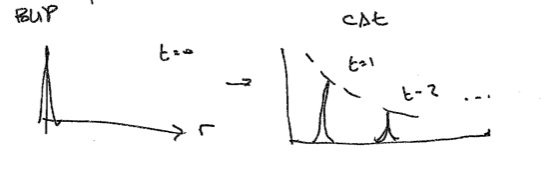
\includegraphics[width=.9\textwidth]{figures/Lec27_3dblip.png}
\end{center}

With a little bit of thought\footnote{This addresses the point in Exercise~\ref{ex:guess:Greens}.}, you could have \emph{guessed} down this Green's function for the wave equation based on the Green's function from the Poisson equation. All you have to do is to remember that the speed of light is constant and you probably want to mathematically enforce causality. In this way, the Poisson equation, the harmonic oscillator, and the wave equation are all \emph{the same damn thing}. They're the appropriate second derivative in a given (3+0)-, (0+1)-, and (3+1)-dimensional spacetime.

To pontificate further on this: all of the uglier versions of the Poisson equation and the wave equation in cylindrical and spherical coordinates are just cousins of what we've done here. Sure, you may have to replace your Fourier expansion over nice plane waves with spherical harmonics or Bessel functions. But you know the deal: we never cared much about the basis functions, we just cared about using the \emph{orthonormality} of these \emph{nice} basis functions to read off the coefficients ($\tilde G$) so that it's easy to represent the solution. Keep this in mind and you won't get lost when you get to the mathematically more tedious examples in your electrodynamics course---you're doing nothing more and nothing less than the harmonic oscillator in some number of dimensions and in some choice of basis.

\begin{exercise}
Solve for the Green's function of the wave equation in (2+1)-dimensional spacetime. Notice that the behavior is quite different from the one in (3+1)-dimensions. Comment on the physics of waves in \emph{Flatland}.
\emph{Answer}:
\begin{center}
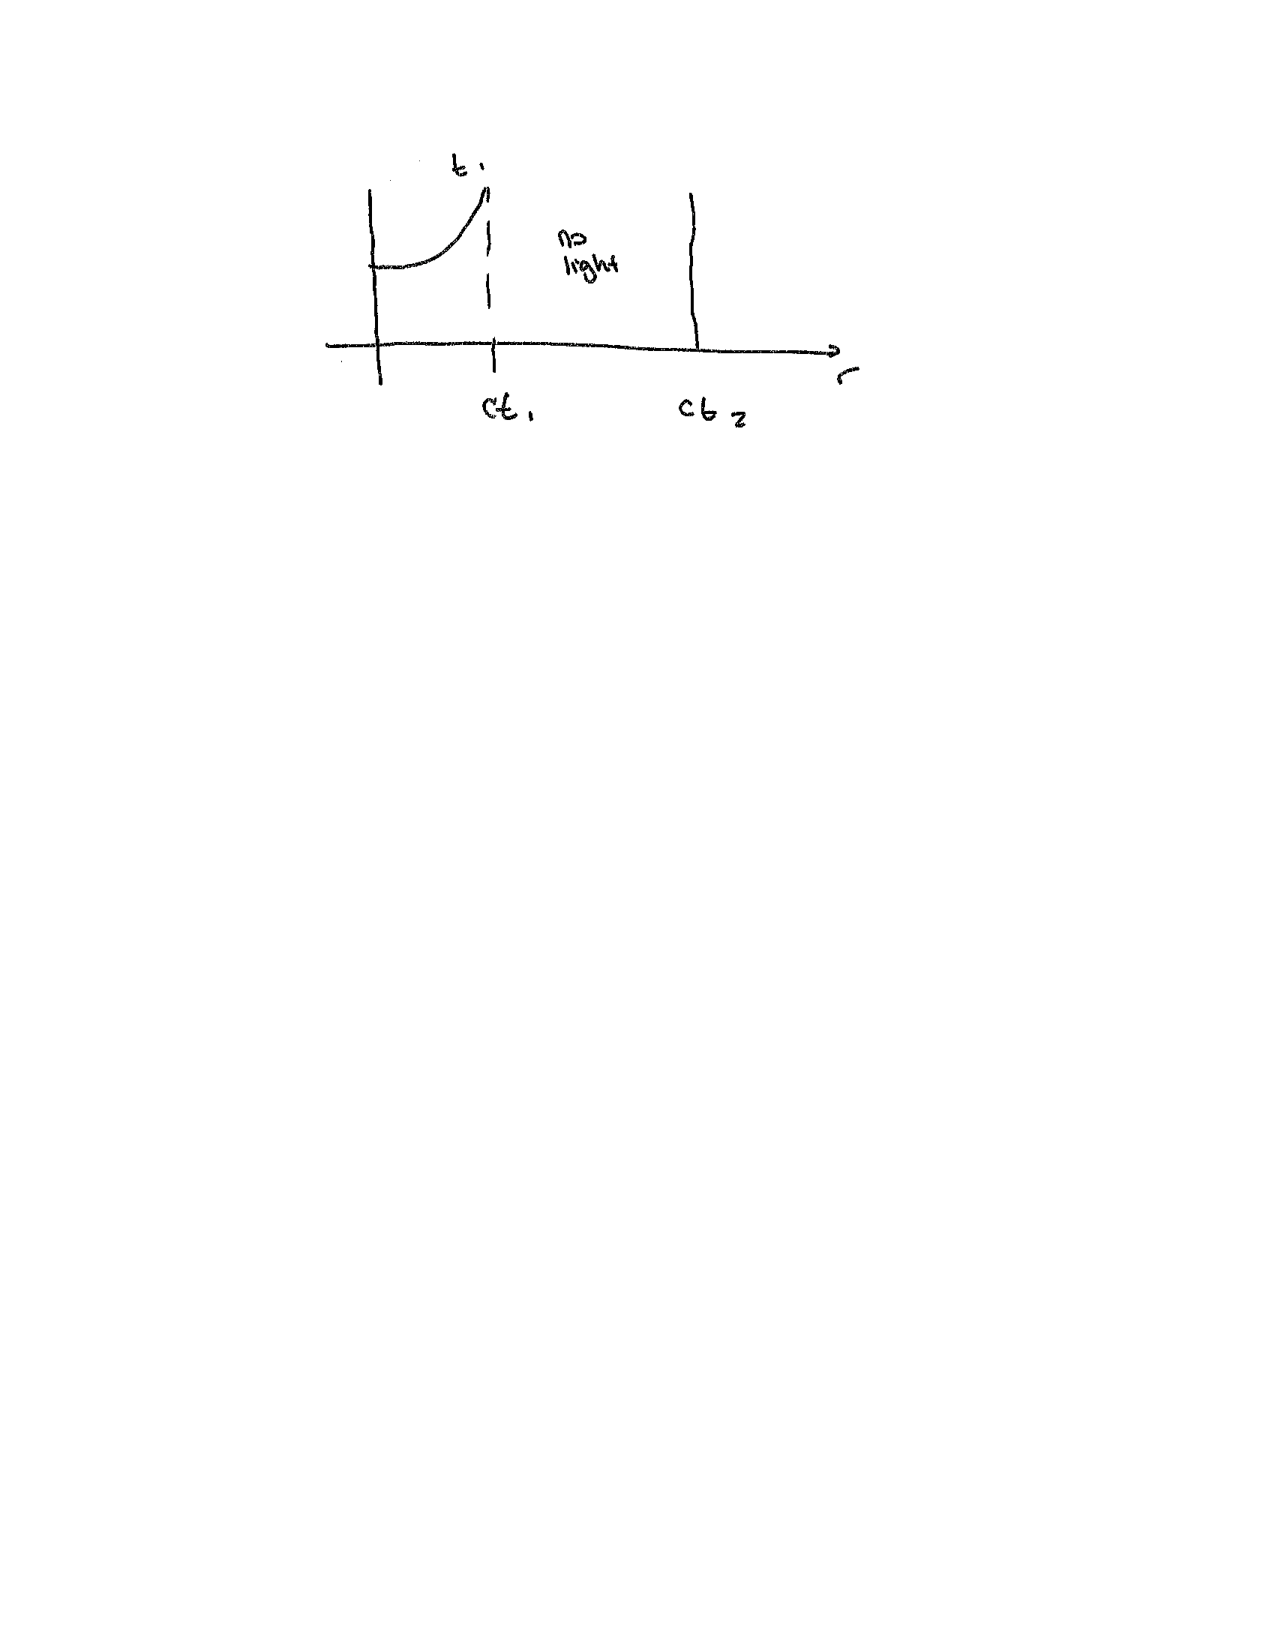
\includegraphics[width=.47\textwidth]{figures/Lec27_2da}
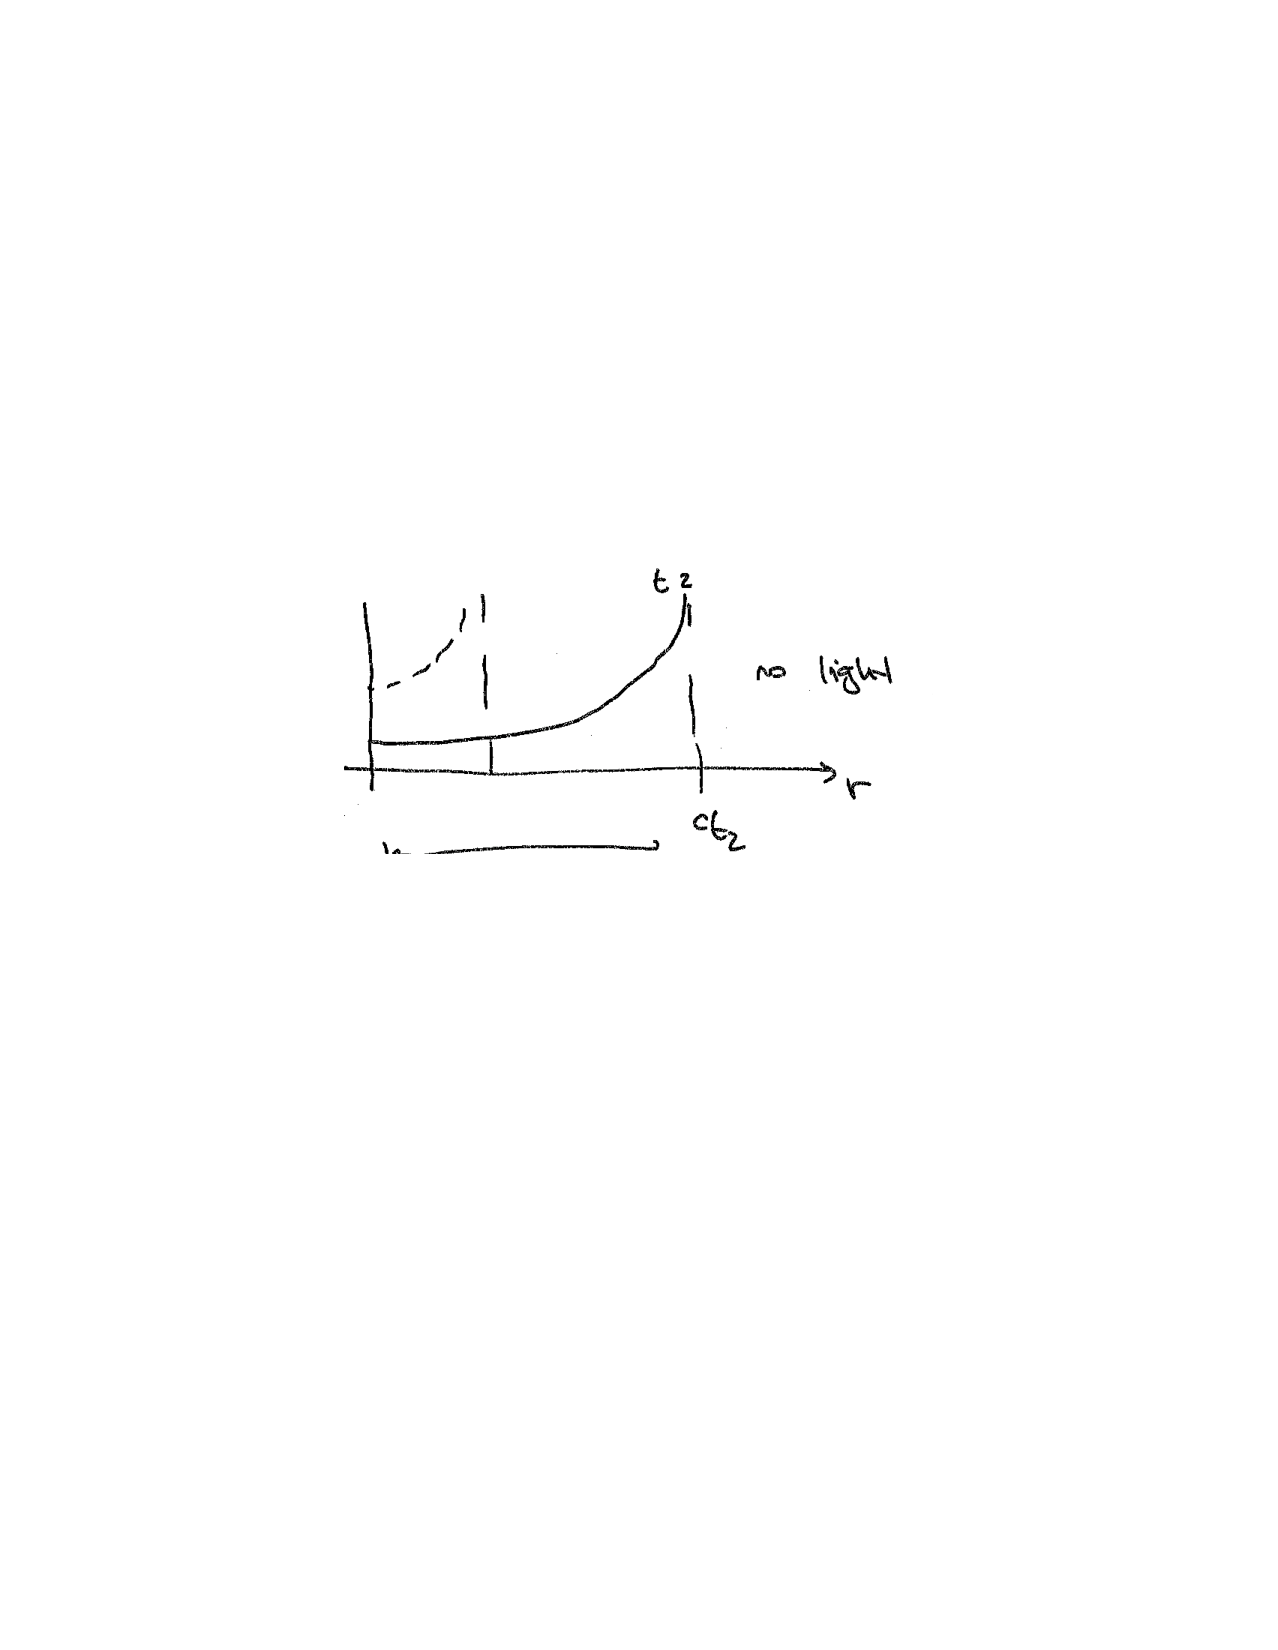
\includegraphics[width=.47\textwidth]{figures/Lec27_2db}
\end{center}
\end{exercise}


\section{Dimensional Reduction}

You can guess that the (2+1)-dimensional Green's function is a different beast. In (3+1) dimensions, we have $\nabla^2 (-1/4\pi r) = \delta^{(3)}(\vec{x})$. On the other hand, in (2+1) dimensions we have $\nabla^2 (\ln r)/(2\pi) = \delta^{(2)}(x)$, where the $\nabla^2$ is the appropriate spatial d'Alembertian in each case.

\begin{exercise}
Do you remember deriving the $\varphi\sim \ln r$ potential somewhere? I think most students must have done this, but perhaps not explicitly in the guise of Green's functions in flatland.
\end{exercise}

\begin{exercise}
What are the dimensions of $G_{(2+1)}$? How do these compare to the dimensions of $G_{(3+1)}$? Keep track of this difference as we go over this section.
\end{exercise}

There is a clever way to deduce the (2+1)-dimensional Green's function. In fact, one could have used this trick to derive the (3+1)-dimensional Green's function from the 3-dimensional Green's function. We propose that
\begin{align}
  G_{(2+1)}(t,x,y) &= \int_{-\infty}^\infty dz\, G_{(3+1)}(t,x,y,z) \ .
\end{align}
That is: we integrate out the extraneous dimension from the higher-dimensional Green's function. To see this, insert the Fourier representation of $G_{(3+1)}$:
\begin{align}
  \int_{-\infty}^\infty dz\, G_{(3+1)}(t,x,y,z)
  &=
  \int dz\,\dbar^4k\, e^{-iEt+i\vec{k}\cdot\vec{x}} \tilde G_{(3+1)}(E,k_x,k_y,k_z) \ .
\end{align}
We can perform the $dz$ integral: $\int dz \,e^{ik_zz} = 2\pi \delta(k_z)$. This gives
\begin{align}
  \int_{-\infty}^\infty dz\, G_{(3+1)}(t,x,y,z)
  &=
  \int \dbar^3k\, e^{-iEt+ik_xx+ik_yy} \tilde G_{(3+1)}(E,k_x,k_y,0) \ .
\end{align}
We can now plug in the form of $\tilde G_{(3+1)}$:
\begin{align}
  \tilde G_{(3+1)}(E,k_x,k_y,0) &=\frac{1}{E^2-k_x^2-k_y^2} = \tilde G_{(2+1)}(E,k_x,k_y) \ .
\end{align}
\flip{check minus signs.} We observe that the (3+1)-dimensional momentum-space Green's function with $k_z=0$ is exactly the (2+1)-dimensional momentum-space Green's function. The difference is how many integrals one performs to go to position space. So we have found that
\begin{align}
  \int dz\, G_{(3+1)} = \int \dbar^3k\, e^{-iEt+ik_xx +ik_y y} \tilde G_{(2+1)}
  \equiv G_{(2+1)} \ .
\end{align}
Thus we have proved our assertion that the (2+1)-dimensional Green's function is an integral of the (3+1)-dimensional Green's function over the `extra' dimension.

We can go ahead and plug in $G_{(3+1)}$ to find
\begin{align}
  G_{(2+1)}(t,x,y) 
  &= \frac{\Theta(t)}{4\pi}\int_{-\infty}^{\infty}dz\,
  \frac{1}{\sqrt{x^2+y^2 + z^2}}
  \delta(\sqrt{x^2+y^2+z^2}-t) \ .
\end{align}
Recall that
\begin{align}
  \delta(f(z)) &= \sum_{z_0} \frac{1}{|f'(z_0)|} \delta(z-z_0) \ ,
\end{align}
where the sum is over zeros of the function, $f(z_0)=0$. For our case we have $f'(z) = z/\sqrt{x^2+y^2+z^2}$ with zeros at $z_\pm = \pm \sqrt{t^2 - x^2+y^2}$. Using the $\Theta(t)$ to remove an unphysical term, we have
\begin{align}
  G_{(2+1)}(t,x,y) &= \frac{\Theta(t)}{2\pi} \frac{1}{\sqrt{t^2-x^2-y^2}} \ .
\end{align}


The following figures give a bit of intuition for this solution relative to an infinite line charge:
\begin{center}
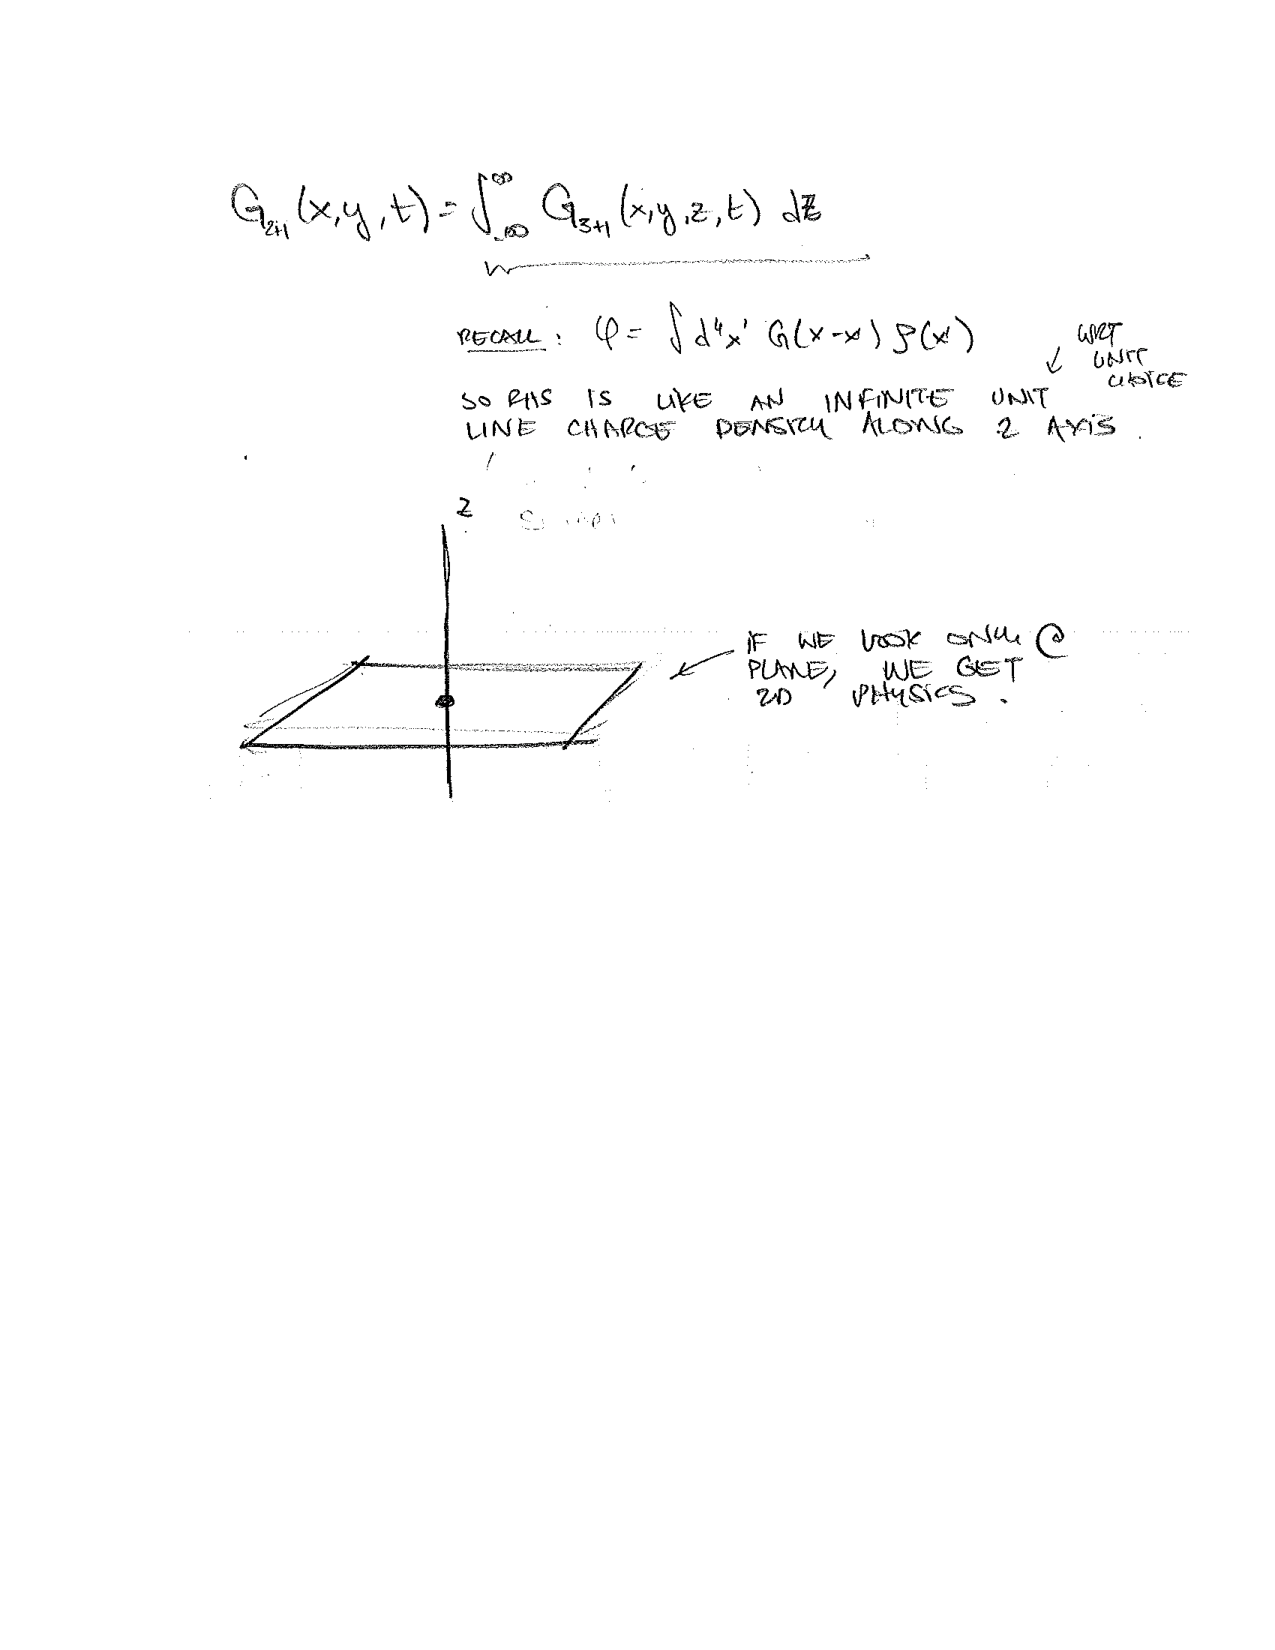
\includegraphics[width=.47\textwidth]{figures/Lec08_XD_2D1}
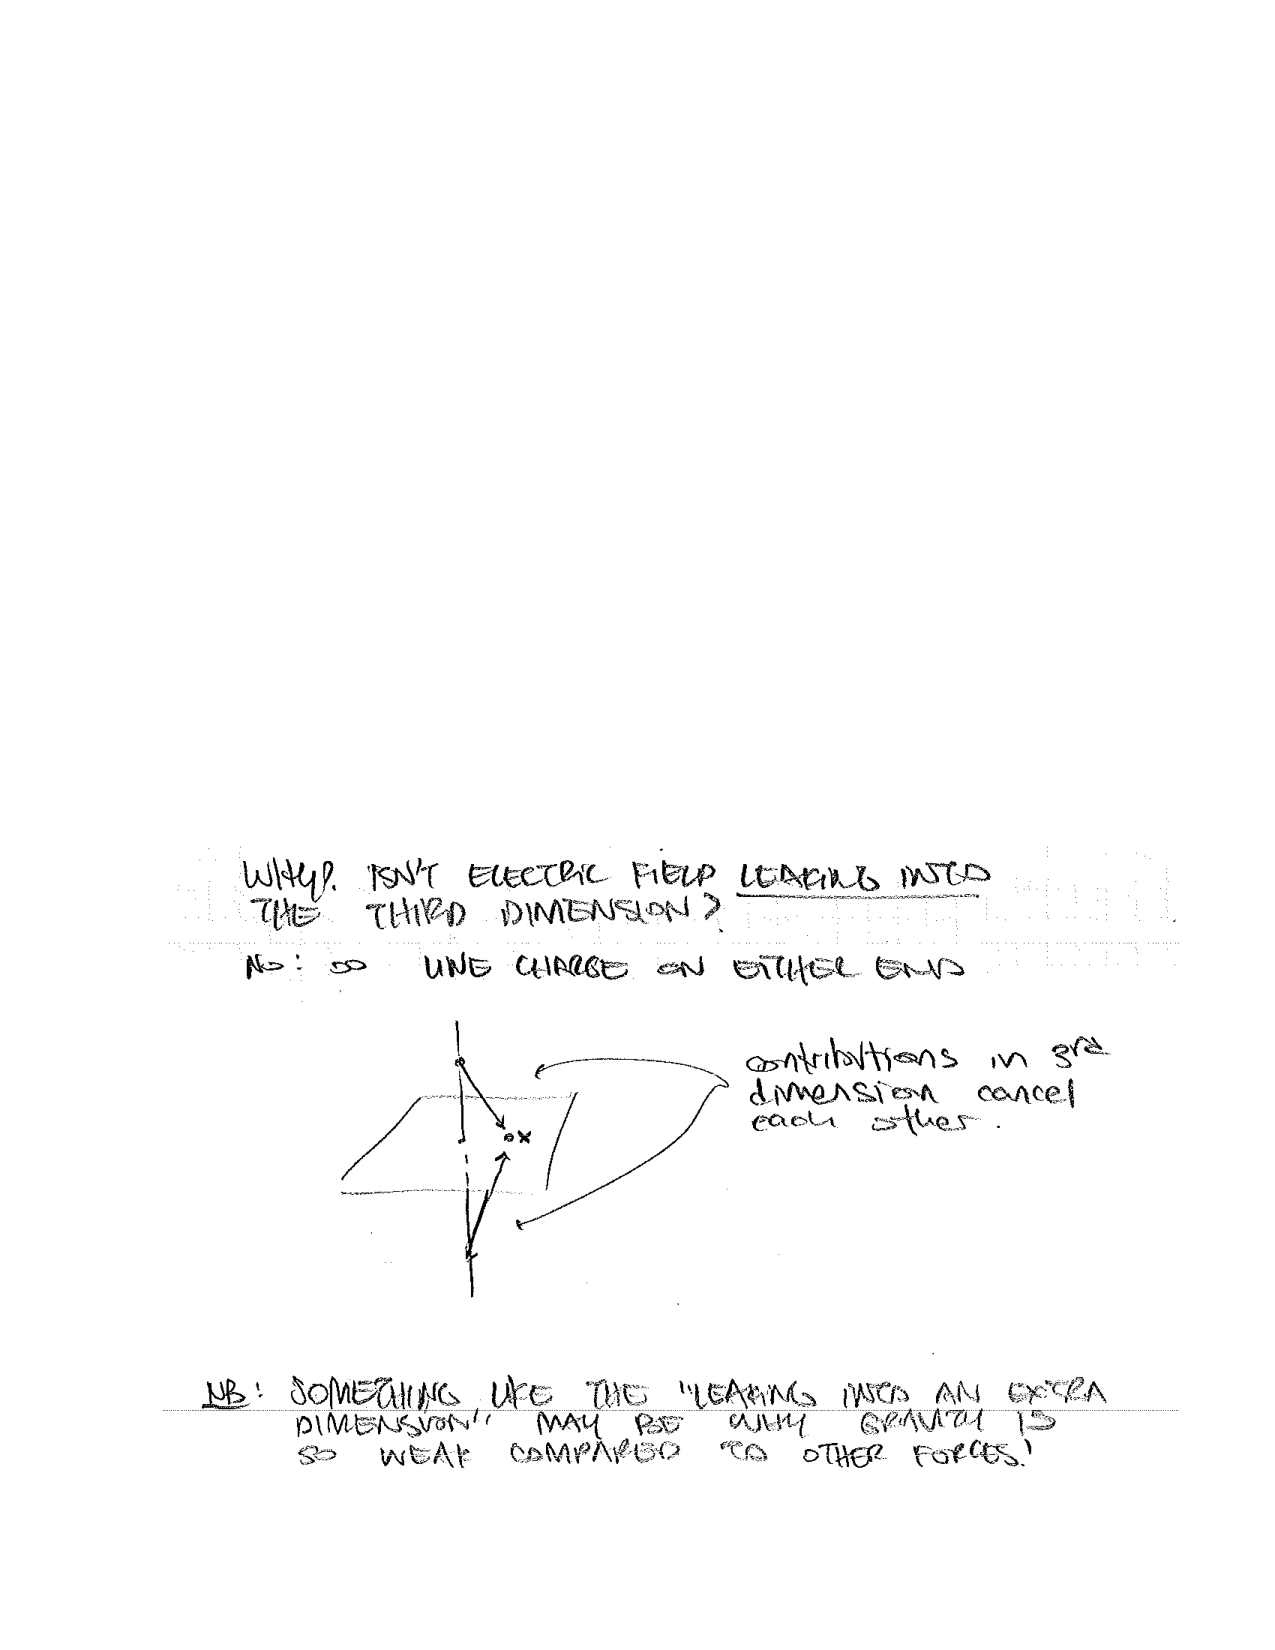
\includegraphics[width=.47\textwidth]{figures/Lec08_XD_2D2}
\end{center}
The key insight is that $\int dz\, G_{(3+1)}$ is precisely the form of the potential coming from an infinite, uniform line charge extending in the $z$-direction from the origin. The electric field would ordinarily `leak' into the extra dimension, but the infinite line charge cancels the potential that leaks off of a given sheet. Note that by symmetry the non-trivial potential profile is restricted to the plane.



\begin{exercise} Application to biophysics. Derive the position-space two point function in equation (3.17) of \texttt{cond-mat/9601006v2}\footnote{\url{https://arxiv.org/abs/cond-mat/9601006v2}}. One has to perform a two-dimensional (inverse) Fourier transform to show: 
\begin{align}
  \int \dbar^2p 
  \frac{ e^{i \vec{p} \cdot (\vec{x}-\vec{y}) } }{p^4}
  &=
  \frac{1}{16\pi} R^2 \ln R^2 \ ,
\end{align}
where $\vec{R} = \vec{x}-\vec{y}$ and $R = |\vec{R}|$. The dot product in the exponential gives the cosine of an angle. If we move to polar coordinates in momentum space, we get $p\,dp\,d\theta$. Because the two-dimensional measure is $d\theta$ rather than $d\cos\theta$, this integral is somewhat tricky. Derive the above result by performing the analogous integral in \emph{three} dimensions and then dimensionally reducing to two dimensions. 
\emph{Thanks to Yankang Liu (P232 Fall 2022) for bringing up this application.}
\end{exercise}



